\documentclass[12pt]{report}
\usepackage[utf8]{inputenc}
\usepackage{graphicx}
\usepackage[margin=1.0in]{geometry}
\usepackage{float}
\usepackage{subfig}\usepackage[hyphens]{url}
\usepackage[hidelinks]{hyperref}
\hypersetup{breaklinks=true}
\urlstyle{same}
\usepackage{cite}
\usepackage{fancyhdr}
\pagestyle{fancy}


% this is to fix header confusion 
\newcommand{\sectionWithFixedHeader}[2]{\section[#1]{#1\sectionmark{#2}}\sectionmark{#2}} 
                    % \sectionWithFixedHeader{Long title}{Short title}


\graphicspath{ {images/} }

\title{{Upgrades to the ALICE Fast Interaction Trigger T0+ A-side Hardware and Simulations}\\
{\large Department of Physics, California Polytechnic State University}\\
{\large San Luis Obispo}\\
}
\author{Joe Crowley}
\date{June 2020}
 
\begin{document}


\maketitle
\begin{abstract}
	As the Large Hadron Collider is shut down for its second upgrade period, the ALICE collaboration has been performing upgrades on detectors and computing systems. Electronics for T0+ were assembled and tested and will be in use in the ALICE cavern during Run 3 of the LHC. Simulations of T0+ will be used to better reconstruct tracks, account for background contributions, and improve multiplicity and centrality resolution of the Fast Interaction Trigger. Some examples of future work based on this project are given at the end of the manuscript, including hardware and software tasks that will introduce students to high-energy physics in an impactful and lasting learning experience.
\end{abstract}

\tableofcontents

\chapter{Introduction}

\section{Quantum Chromodynamics}
Relativistic deep-inelastic collisions of large ions produce high-energy interactions that allow for studies of High Energy Density (HED) matter. HED matter studied at ALICE from p-p, Pb-Pb, and Xe-Xe collisions is a mess of standard model particles called the Quark-Gluon Plasma (QGP). QGP is a medium of strongly-interacting particles that can reach temperatures higher than $10^{12}$ Kelvin, where the energy density is so high that interactions produce quarks that are asymptotically free. This is in the perturbative domain of quantum chromodynamics (QCD) because quarks and gluons are separated by short distances and have large exchanges of momentum, reducing the effect of gluonic self-interactions.
As the QGP expands, the energy density reduces and asymptotic freedom is no longer an appropriate approximation. Hadrons in the QGP interact to form baryons and mesons during cooling, a process referred to as rehadronization. The newly formed quark matter expands and produces jets that lose energy as they interact with the QGP. The energy loss of the jets as they traverse the QGP is known as jet quenching, and studying this process is critical to understanding the gaps between perturbative and lattice QCD. Heavy ion collision experiments are at the frontier of the high-energy region of the phase space for QGP. Fig. \ref{fig:QGP_Phase_Diagram} shows the phase diagram for QGP in terms of the Baryochemical Potential $\mu_B$ and the Temperature. 

\begin{figure}
    \centering
    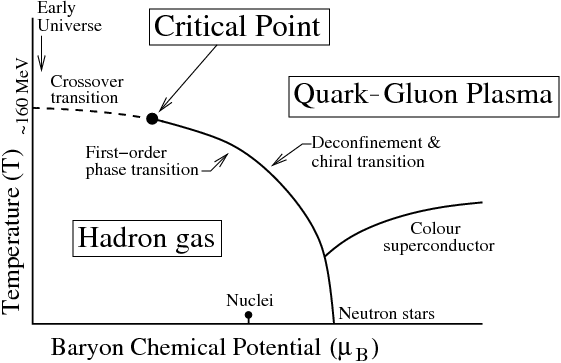
\includegraphics[width=0.6\textwidth]{figures/ALICE/QGP_Phase_Diagram.png}
    \caption{Phase diagram for the Quark-Gluon Plasma. Accelerator experiments with heavy ions allow for the exploration of the phase transitions between Hadron Gas and QGP. 1 MeV$\sim 10^{10}$K 
    cite $https://cds.cern.ch/record/1695331/plots$}
    \label{fig:QGP_Phase_Diagram}
\end{figure}


\section{CERN Large Hadron Collider}
\begin{figure}[H]
    \centering
    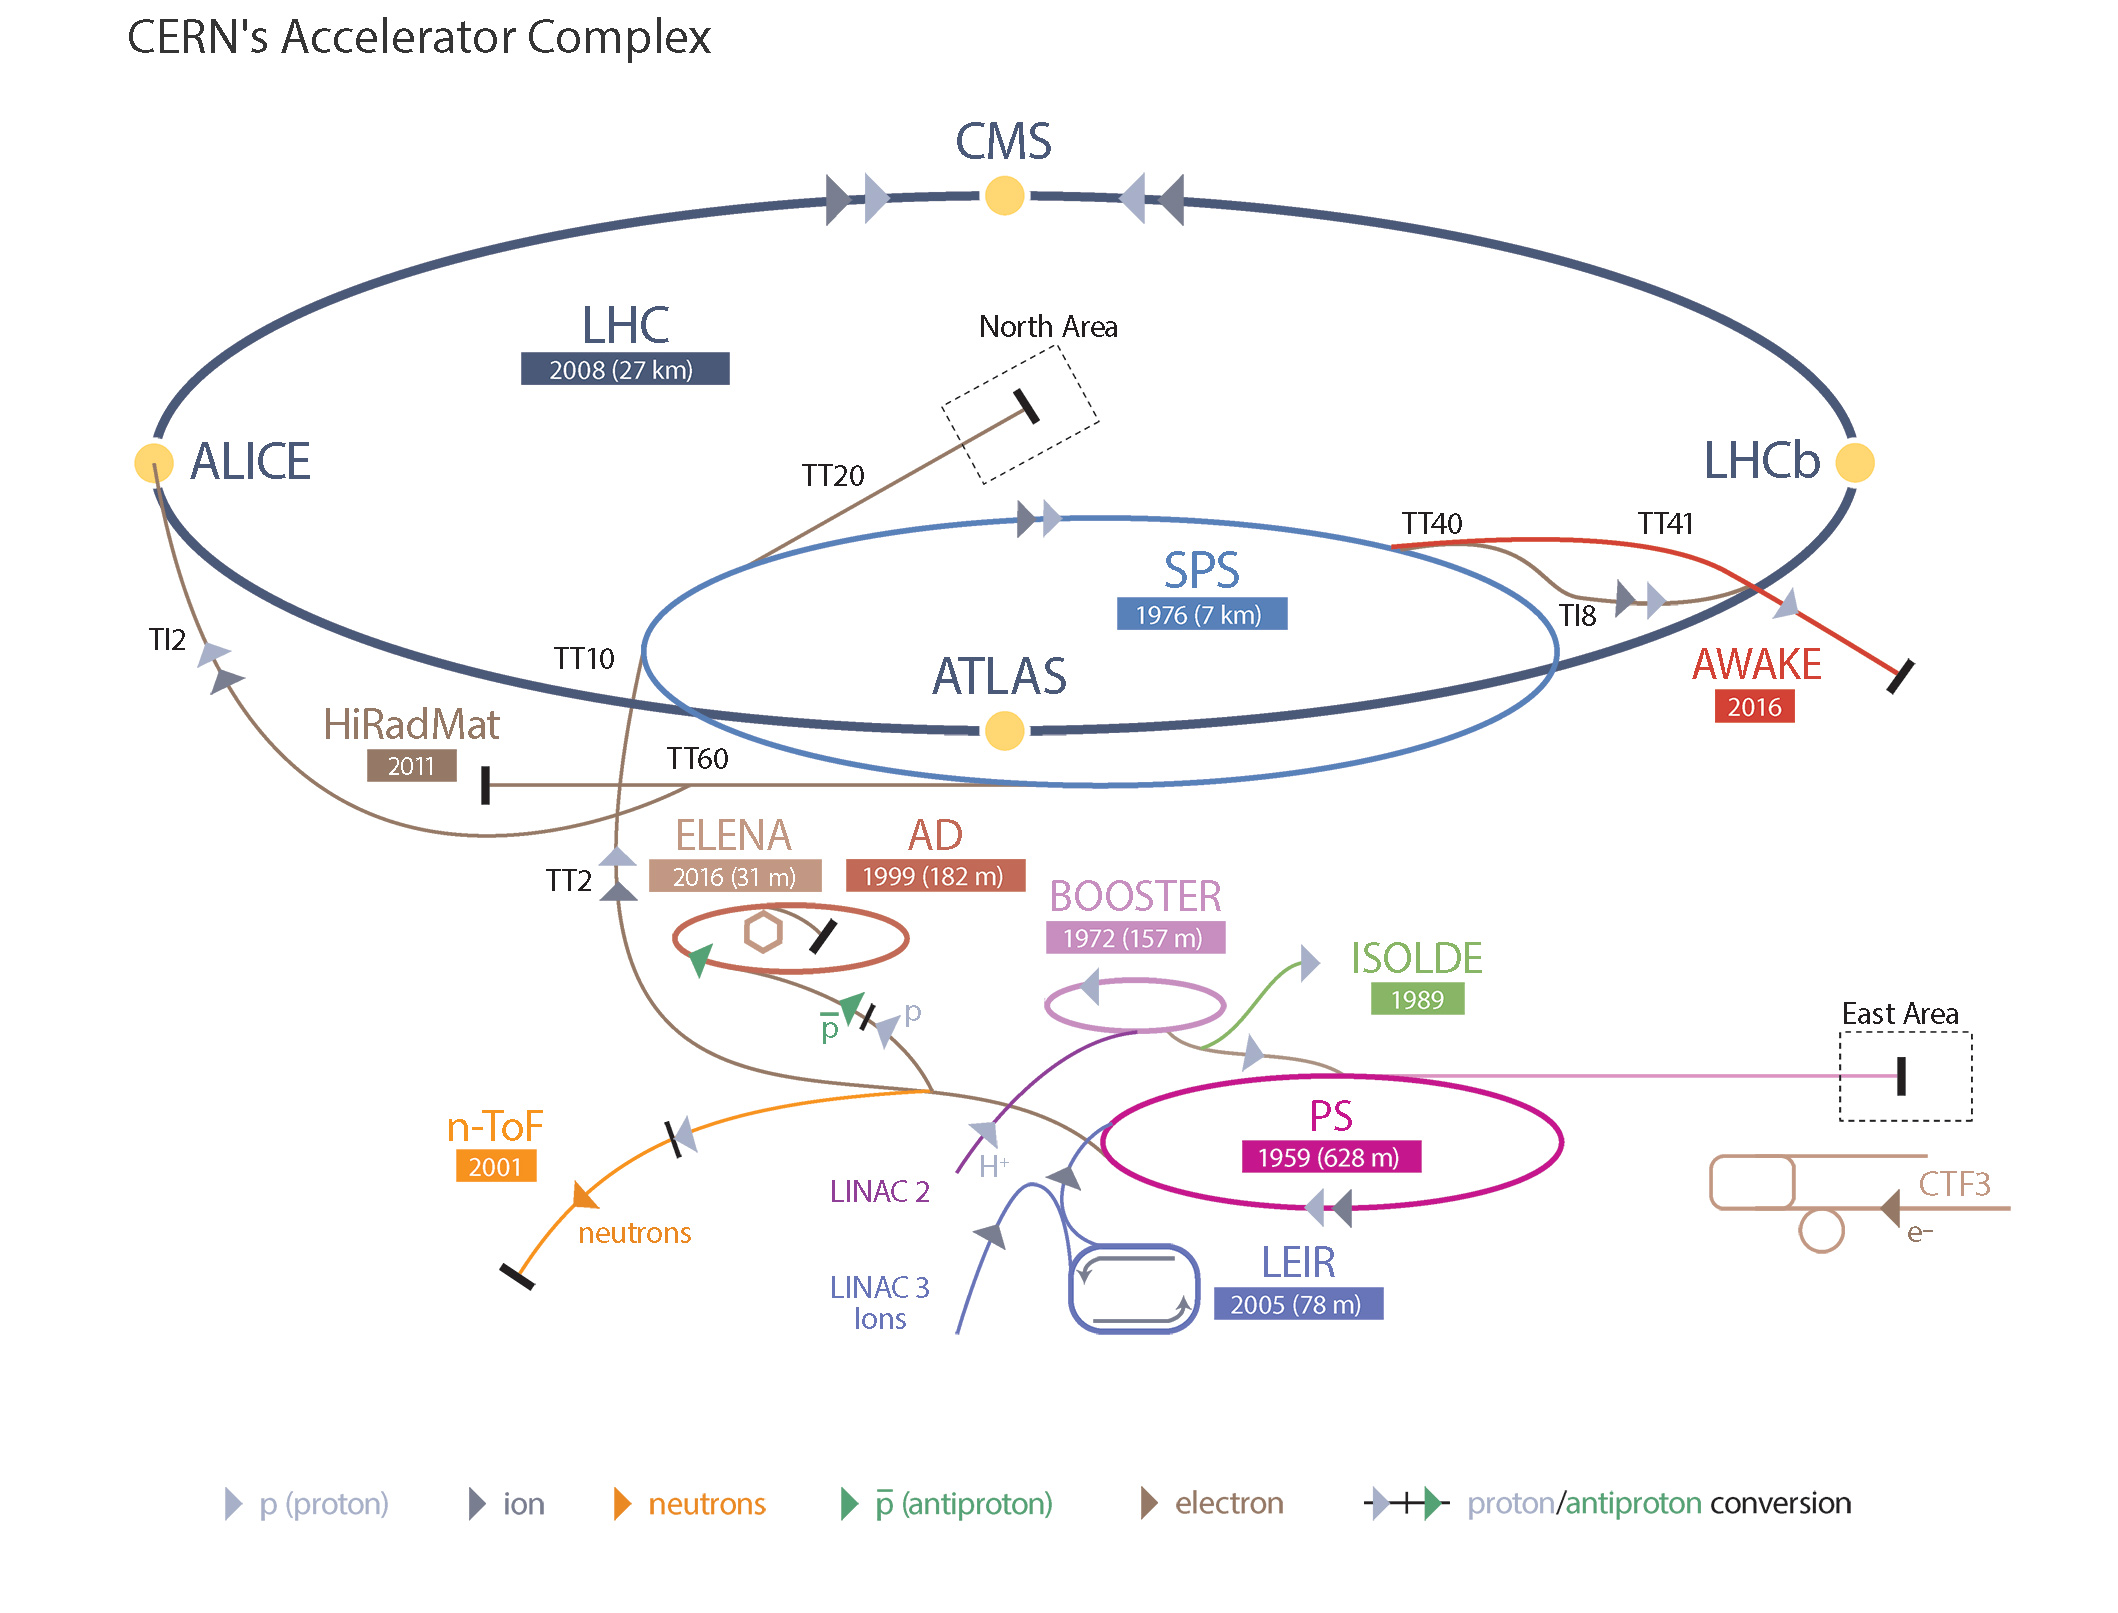
\includegraphics[width=0.7\textwidth]{figures/CERN/LHC_accelerator_complex.jpg}
    \caption{Accelerator complex at CERN Large Hadron Collider}
    \label{fig:CERN_Accelerator_Complex}
\end{figure}

The European Counsel for Nuclear Research (CERN) is one of the largest scientific organizations in the world, where scientists are engaged in the study of the fundamental constituents of the universe. This exploration of the smallest length and time scales is done using the most advanced technology available. CERN's Large Hadron Collider is a collection of accelerator-based experiments that study the way particles interact at very high energies, which gives us clues about the fundamental laws of physics. 

The Large Hadron Collider (LHC) is a 27 km ring of superconducting magnets and accelerating cavities first turned on in September 2008. Particle bunches are accelerated in opposite directions and countercirculate around the ring at energies of up to 7 TeV, guided by magnets cooled to near 1 Kelvin using liquid helium, far colder than space. The particles are then directed to one of four main experiments on the LHC: ALICE, ATLAS, CMS, and LHCb. Each experiment has a detector-based tracking system that measures information about collisions such as energy, position, transverse momentum, centrality, and multiplicity. The LHC accelerator complex is shown in Fig. \ref{fig:CERN_Accelerator_Complex}.

CERN uses the data collected by these experiments to search for new interactions and fields like the Higgs. The data throughput of the LHC is huge; thousands of scientists spend months to years analyzing the data produced by the experiments at the LHC, often to reduce the parameter space of a proposed interaction mode, or to discover and test completely new physics.

Currently, LHC is in its second Long Shutdown (LS2), where scientists upgrade and replace many of the accelerator and detector components. LHC Run 3 will begin in 2021 and continue until 2025. The long term schedule for the LHC is shown in Fig. \ref{fig:CERN_Timelne}.
\begin{figure}[H]
    \centering
    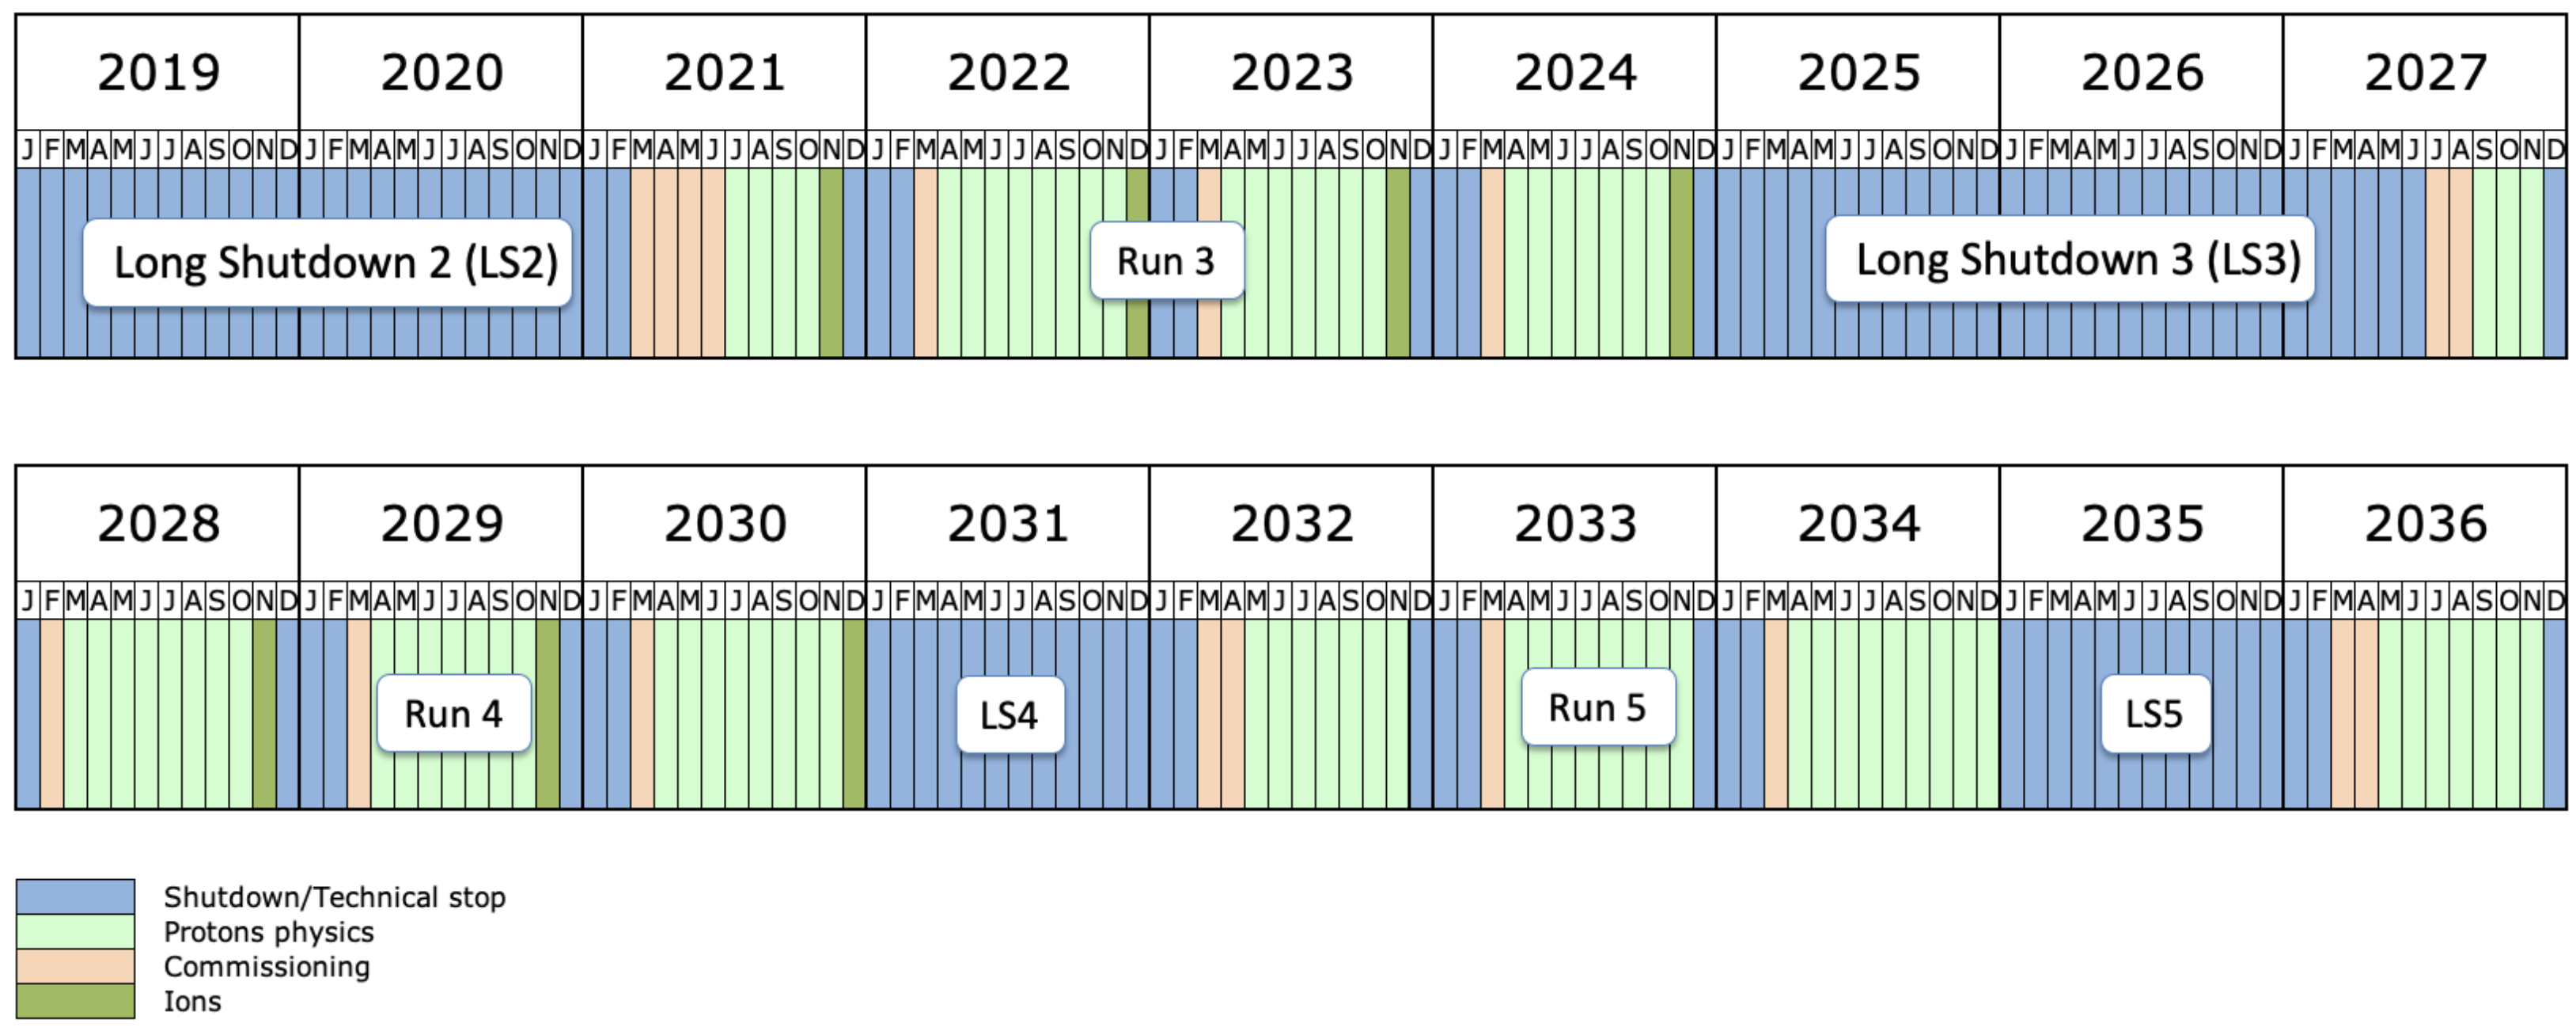
\includegraphics[width=\textwidth]{figures/CERN/LHC_Timeline.png}
    \caption{Long term schedule for LHC from 2019 through 2036.}
    \label{fig:CERN_Timelne}
\end{figure}

\section{A Large Ion Collider Experiment}

\begin{figure}[H]
    \centering
    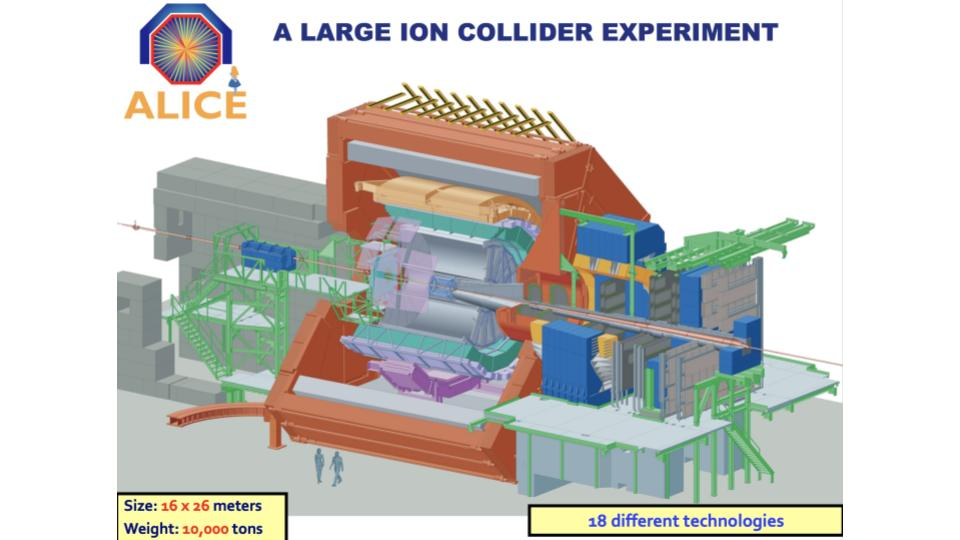
\includegraphics[width=0.6\textwidth]{figures/ALICE/alice_detector.jpg}
    \caption{Schematic cross-sectional view of the ALICE detector system}
    \label{fig:ALICE_DETECTOR}
\end{figure}

ALICE is one of the four main experiments at the LHC. ALICE studies the QGP and strong interactions by detecting and tracking partons, measuring centrality, multiplicity, and energy of collisions. Tracking jets and rehadronization processes as they occur in the detector is incredibly difficult, but we observe the outcome of these processes using a variety of detectors including cerenkov photomultipliers, scintillators, pixel trackers, and calorimeters. Along with L3, the largest normal-conducting magnet in the world, this experiment is at the intersection of advanced technologies and impressive engineering feats. 


\section{ALICE Fast Interaction Trigger}
Hardware triggers based on event multiplicity, transverse momentum, and calorimeter energy provide
event selectivity that allows sampling of the full luminosity of particle beams that collide at ALICE. To study the QGP, event selection requires a minimum bias trigger. In ALICE, this trigger is called FIT, the Fast Interaction Trigger. FIT is a system of detectors that measure the key parameters to determine whether a signal that we pick up is worth tracking; if the appropriate combination of multiplicity, energy, location, time, and transverse momentum are measured, FIT sends a signal to other detectors in ALICE to begin data acquisition (DAQ). Fig. \ref{fig:FIT_IN_ALICE} shows two of the subdetectors within FIT as they are positioned in ALICE. 

\begin{figure}[H]
    \centering
    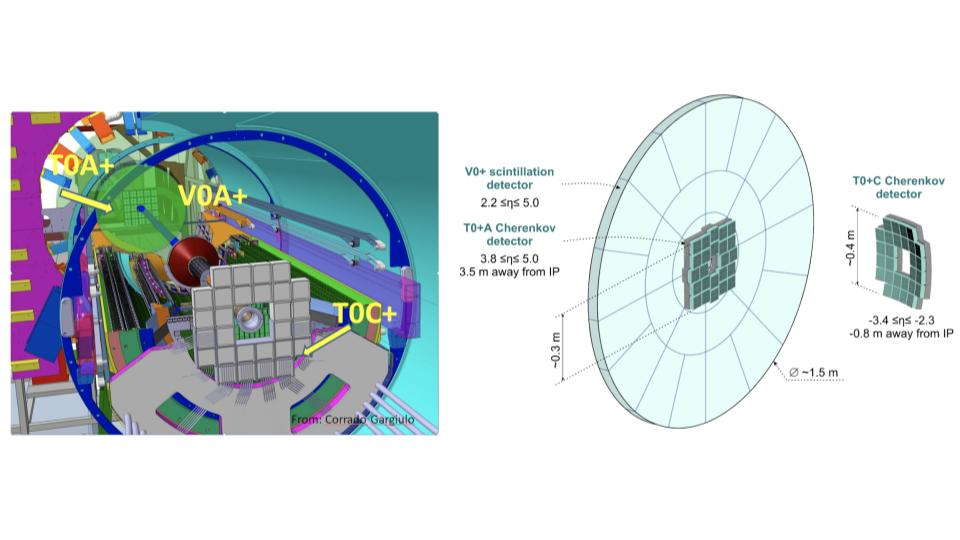
\includegraphics[width=0.6\textwidth]{figures/ALICE/FIT_in_ALICE.jpg}
    \caption{Fast Interaction Trigger positioned inside ALICE, shown in perspective view (left) and in component view (right).}
    \label{fig:FIT_IN_ALICE}
\end{figure}

\section{Online-Offline Computing System}

During LHC Run 3, ALICE is expecting an integrated luminosity of 13 ${nb}^{-1}$ of Pb-Pb collisions in minimum bias mode, with an interaction rate of approximately 50 kHz. To capture maximal information, some detector systems are being upgraded for continuous readout to prevent trigger deadtime losses due to event pileup. This increases the data throughput of ALICE up to the order of TB/s, corresponding to a data volume two orders of magnitude greater than Run 1. ALICE has introduced a new computing framework, $O^2$, which is composed of optimized software and large computing facilities that are designed specifically for detection and analysis of physics events.

Continuous readout of some detectors is a drastic difference from previous techniques. Data collection is achieved with many constant data streams to the computing system. Data flows will be separated into Time Frames, regular intervals synchronized with the LHC clock. Because the data are local and independent the triggering process can be performed with parallel computing. This allows for the simultaneous DAQ and processing, which is very useful for data volume reduction. Results are stored in Tier 0 of the CERN data center or in the $O^2$ farm. These results are further processed later using resources from the CERN Grid and are available for analysis to anyone with access to the Grid. Fig \ref{fig:O2_Schematic} shows the flow of data from detector to the grid, along with the iterated compression and reconstruction of data. 


\begin{figure}[H]
    \centering
    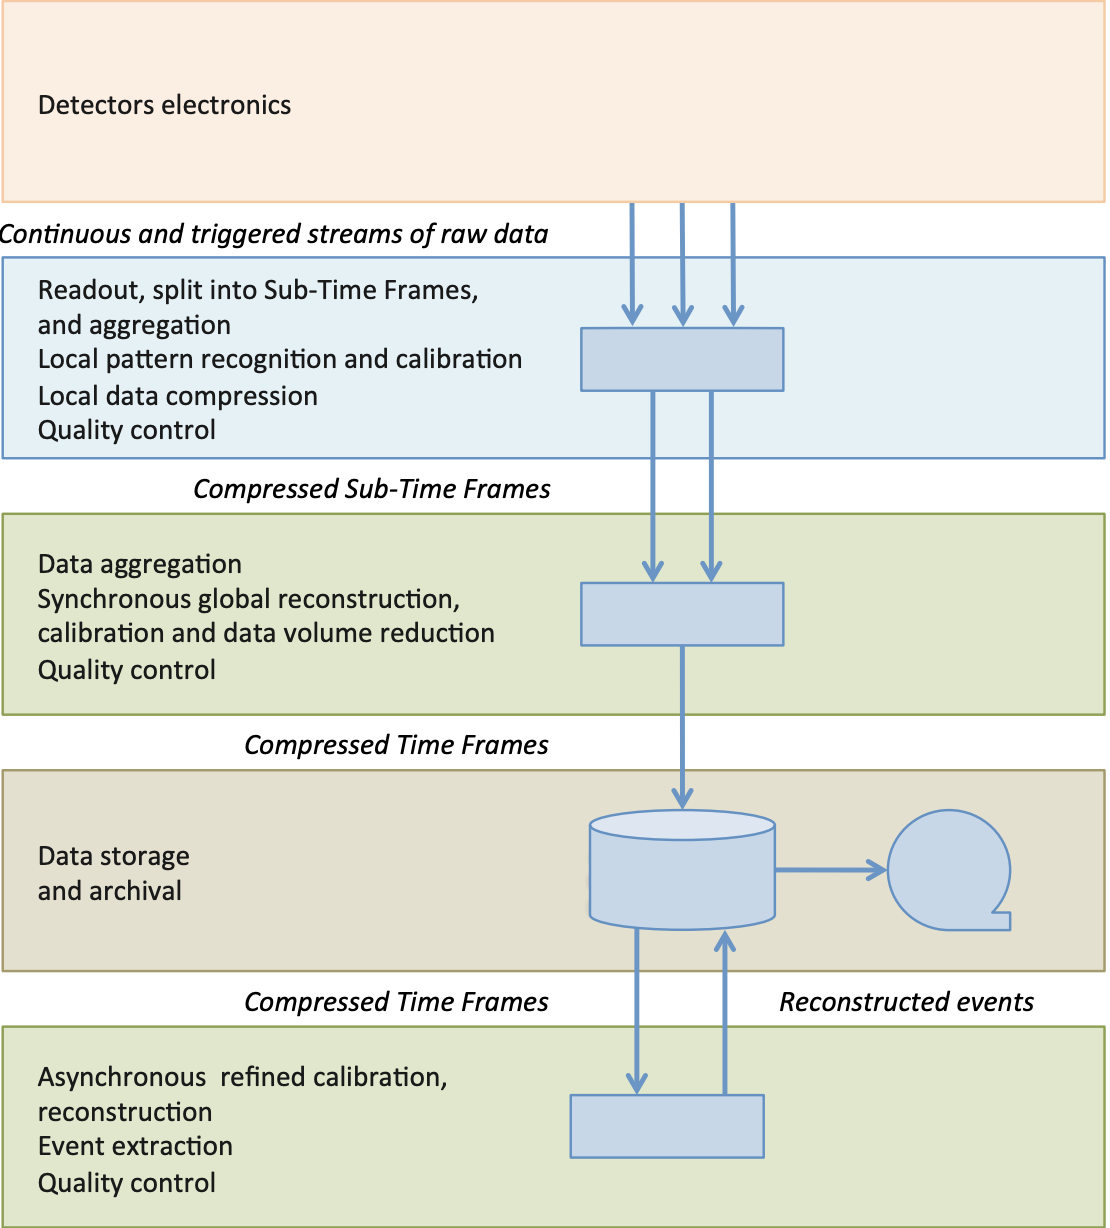
\includegraphics[width=0.6\textwidth]{figures/O2/O2_schematic.png}
    \caption{Diagram of the data flow from the ALICE detectors through the $O^2$ computing system. Compression and reconstruction are iterated until both data size and quality are optimized}
    \label{fig:O2_Schematic}
\end{figure}



\chapter{The FIT T0+ Detector}
The Fast Interaction Trigger is a detector system that measures the fundamental experimental parameters for analyzing particle interactions in ALICE: FIT measures the location and time of interactions, as well as multiplicity and centrality. These parameters are measured using scintillators and Cherenkov detectors. T0+ is a Cherenkov detector composed of crystals and photomultipliers; it measures the location and energy of particles that pass through the crystals. When signals are detected on multiple channels of the detector within a specified time interval, they trigger a signal that initiates data acquisition on other detector systems. This is called a coincidence measurement, and is the first data required in event reconstruction. FIT T0+ (FT0) uses coincidence measurements and channel data to determine the trajectories of particles moving transverse to the beamline.

\begin{figure}[H]
    \centering
    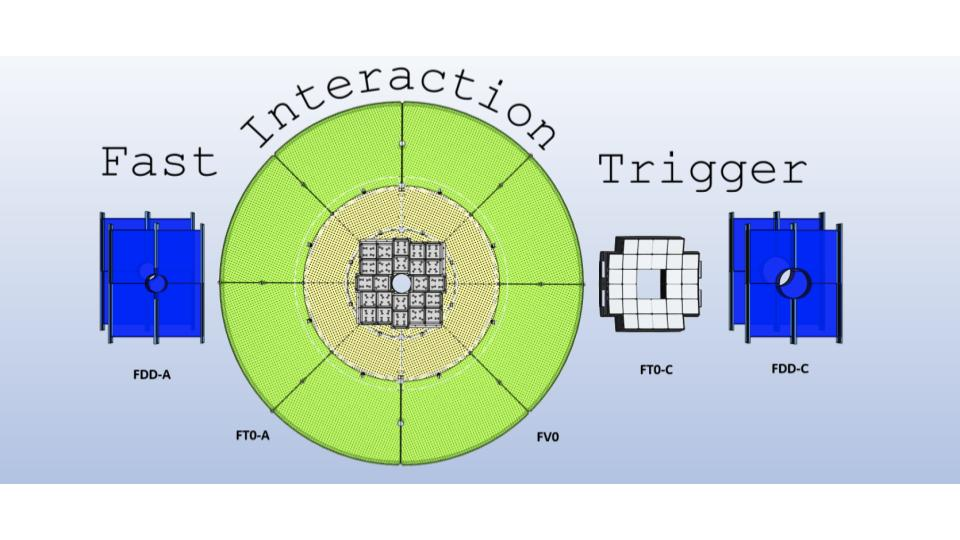
\includegraphics[width=0.6\textwidth]{figures/FIT/FIT_Logo.jpg}
    \caption{Logo for the Fast Interaction Trigger, showing the FDD, FT0, and FV0 detectors.}
    \label{fig:FIT_Logo}
\end{figure}


\section{FIT T0+ Hardware}
T0+ is a Cherenkov detector that consists of two sides, A and C. A-side and C-side sit on opposite ends of the interaction point to increase the precision of measurements on interactions that have low transverse momenta. A-side has twenty-four photomultipliers, each with four separate channels. C-side has twenty-eight photomultipliers, which are angled toward the beamline. Together, these Cherenkov detectors are used to measure important beam characteristics and trigger DAQ on other detectors in ALICE. 

\begin{figure}[H]
    \centering
    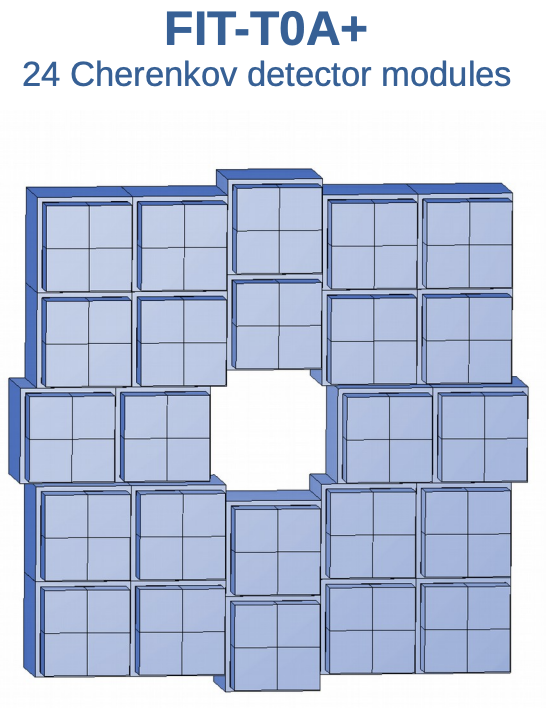
\includegraphics[width=0.4\textwidth]{figures/FIT/FT0A_Structure.png}
    \caption{Structure of the FIT T0+ A-side, with 96 channels across 24 detector modules. cite $https://indico.cern.ch/event/798978/attachments/1796182/2929226/2019.02-Slupecki-IntroToFitElectronics.pdf$}
    \label{fig:my_label}
\end{figure}

\begin{figure}[H]
    \centering
    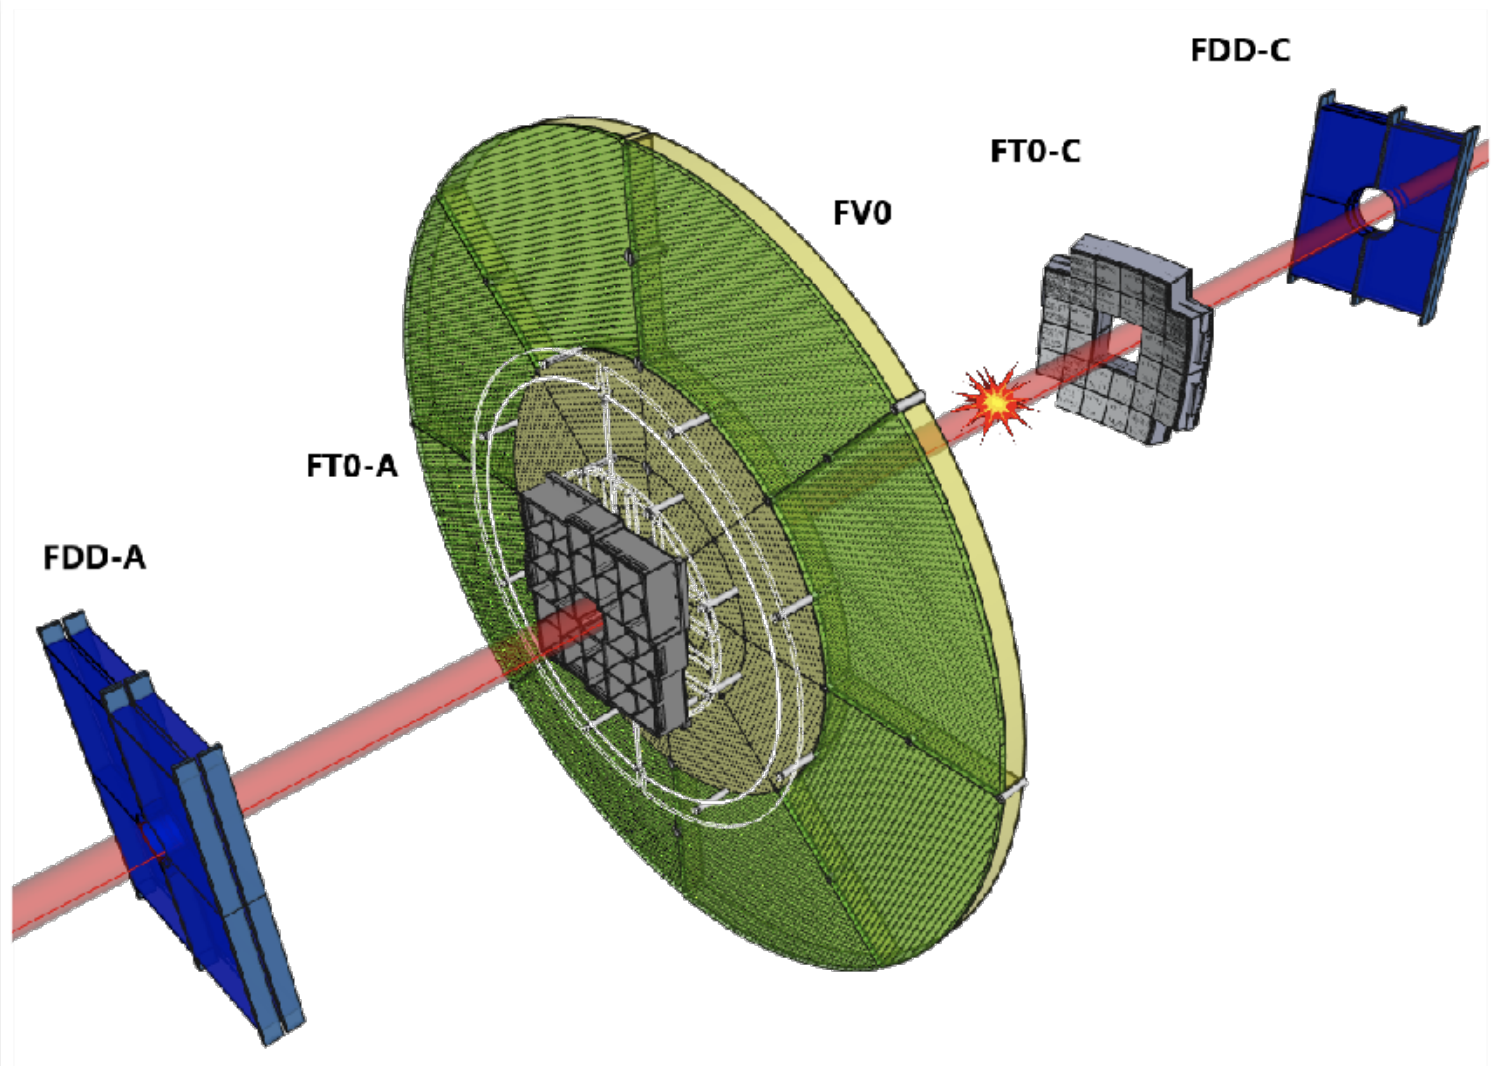
\includegraphics[width=0.6\textwidth]{figures/FIT/FIT_Layout.png}
    \caption{FIT T0+ shown in schematic view with the other detectors in FIT, V0+ and FDD. A-side and C-side are on opposite sides of the interaction point. cite $https://indico.fjfi.cvut.cz/event/110/contributions/2697/attachments/842/1138/Decin2019_jgcn_FDD.pdf$}
    \label{fig:FIT_Layout}
\end{figure}


\subsection{Micro-Channel Plate Photomultiplier Tube}
T0+ measures the location and energy of particles using a Cherenkov radiative quartz material coupled to a photomultiplier. Fast moving particles produce Cherenkov radiation within the quartz, which then hits the photocathode of the PMT. This produces photoelectrons that are accelerated toward metal plates called dynodes, which release more electrons. The acceleration and electron amplification is repeated across high potential differences until there are enough electrons to measure with a picoammeter. Because of this acceleration and amplification process, PMTs require high-voltage, on the order of kV. Micro-Channel Plate Photomultipliers (MCP-PMT) differ from regular photomultipliers in that they do not have discrete dynodes, instead having thin glass plates with many holes with diameter 1-100$\mu$m. MCP-PMTs are required in ALICE because of their minimal gain loss in strong magnetic fields. Having multiple anodes that read the current passing through provides better spacial resolution than the single-anode PMT. The electronics for the FIT T0 MCP-PMTs are shown in Fig. \ref{fig:MCP_PMT_Schematic}.
\begin{figure}[H]
    \centering
    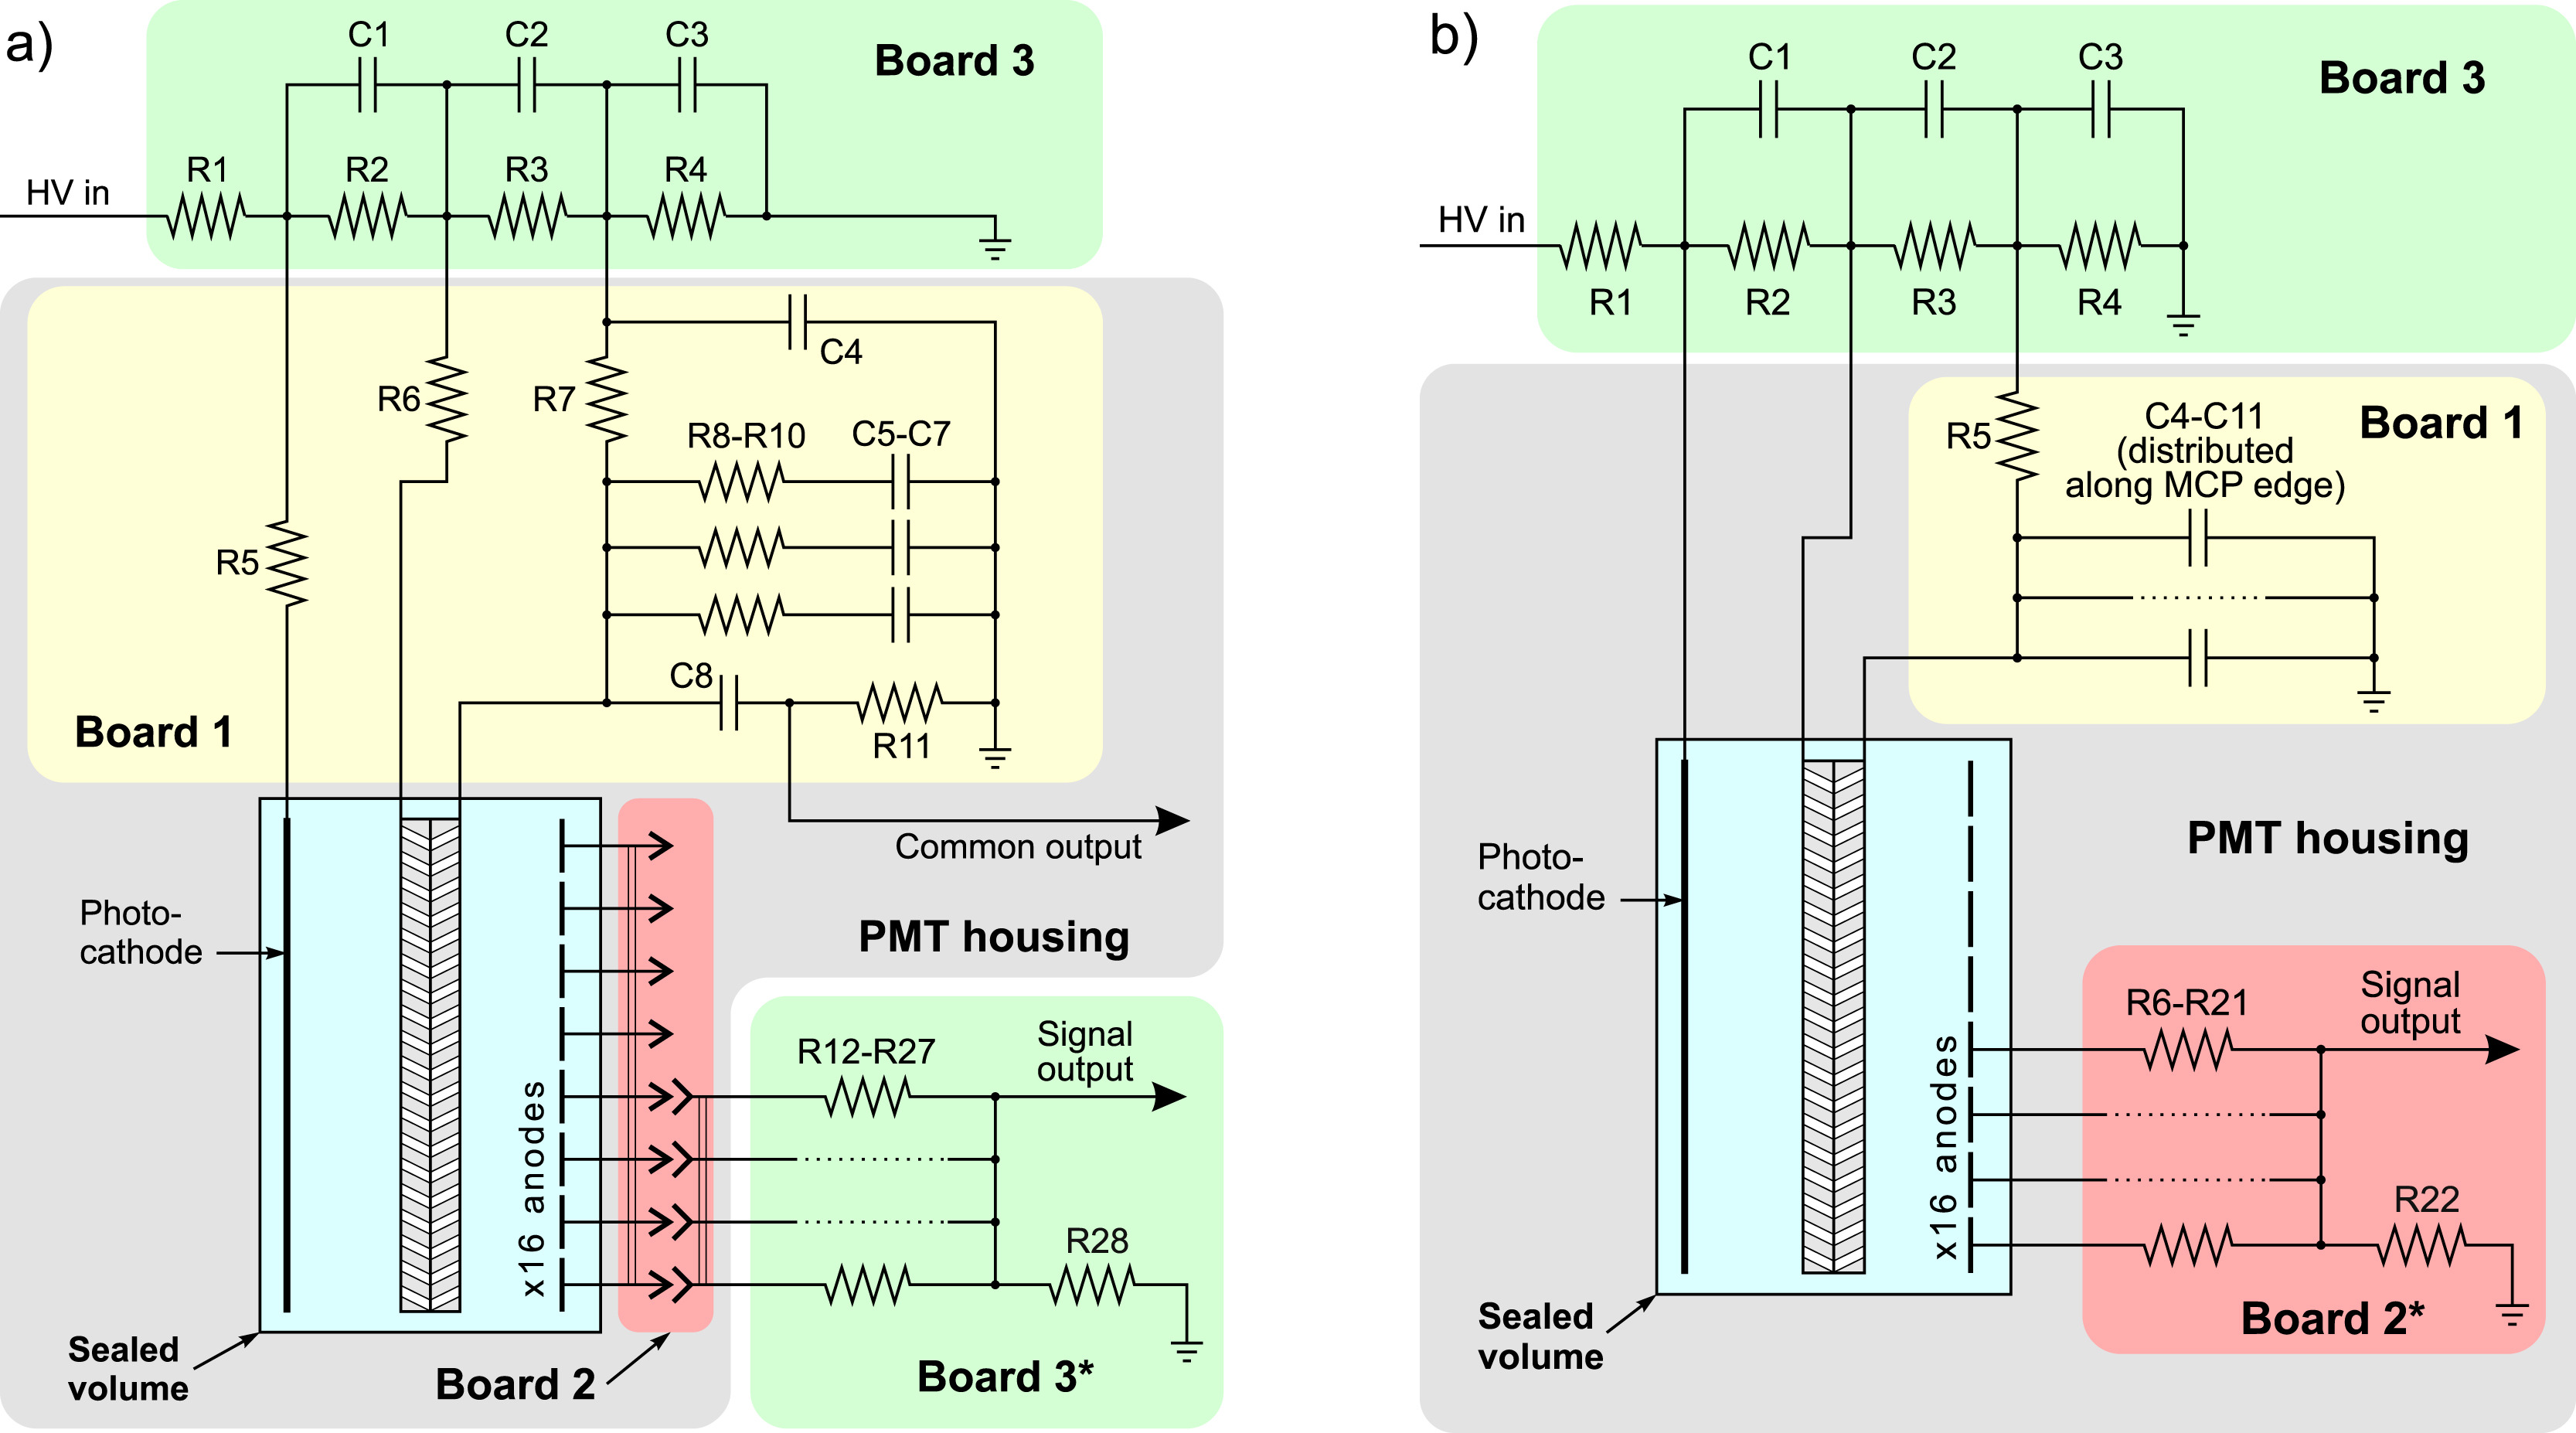
\includegraphics[width=0.8\textwidth]{figures/FIT/PMT_Schematic.jpg} 
    \caption{Schematic for the MCP-PMTs used for the FIT T0+ Cherenkov detector \cite{Yury_MCP-PMT}}
    \label{fig:MCP_PMT_Schematic}
\end{figure}



\sectionWithFixedHeader{High-Voltage Power Electronics for MCP-PMT}{HV PMT Electronics}
MCP-PMTs require large potential differences to create a measurable current from a photon that hits the photocathode. However, if the voltage is too high, then the signal can become saturated, and the resolution of the detector is compromised. Fig. \ref{fig:MCP_PMT_Schematic} shows a schematic view of the MCP-PMTs in FIT. Each PMT is equipped with a voltage divider circuit that takes in a voltage of $\sim$2 kV, and supplies voltage to three of the elements in board one: the photocathode, and on either side of the micro-channel plate. The assembly of the HV power electronics was done in summer of 2019 at the FIT lab at CERN. This includes adding coaxial LEMO connectors to the HV cables and securing the cables to the power board (Board 3 in Fig. \ref{fig:MCP_PMT_Schematic}). The assembled power electronics are shown in Fig. \ref{fig:power_board}.

\begin{figure}[H]
    \centering
    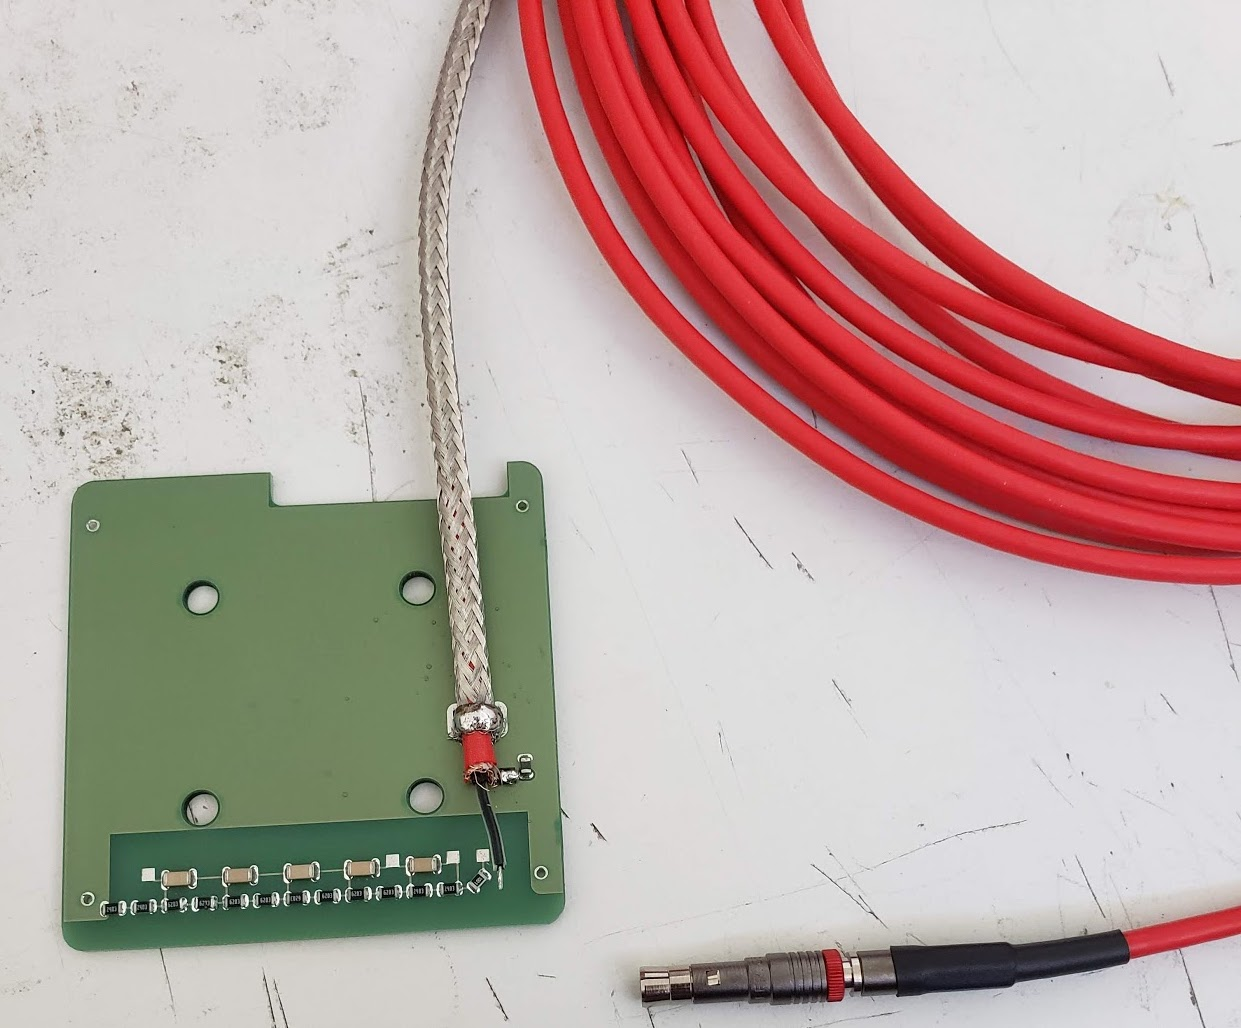
\includegraphics[width=0.6\textwidth]{figures/FIT/power_board.jpg}
    \caption{HV power electronics for MCP-PMT in FIT T0+ A-side}
    \label{fig:power_board}
\end{figure}

\section{MCP-PMT Testing at CERN}\label{pmt_testing}
During LS2, the FIT collaboration has been working on the upgrades to the hardware for T0+, hoping to increase resolution, minimize crosstalk, and maximize the trigger efficiency. This is done using the MCP-PMTs showin in Fig \ref{fig:MCP_PMT_Schematic}, which are split into four channels based on the 16 anodes. Before this hardware is installed in ALICE, it must be tested for optimal performance. To test the most important aspects of MCP-PMT performance, laser pulses are sent to the PMTs to measure the response. The pulses are produced by a laser, then split to have a reference signal. The reference signal is measured on a PMT with well known characteristics. The test signal is sent to one of the PMTs in T0+. By comparing the output current spikes from the reference and the test PMTs, we can test the performance of PMTs as they are shipped from Hamamatsu. 


\begin{figure}[H]
    \centering
    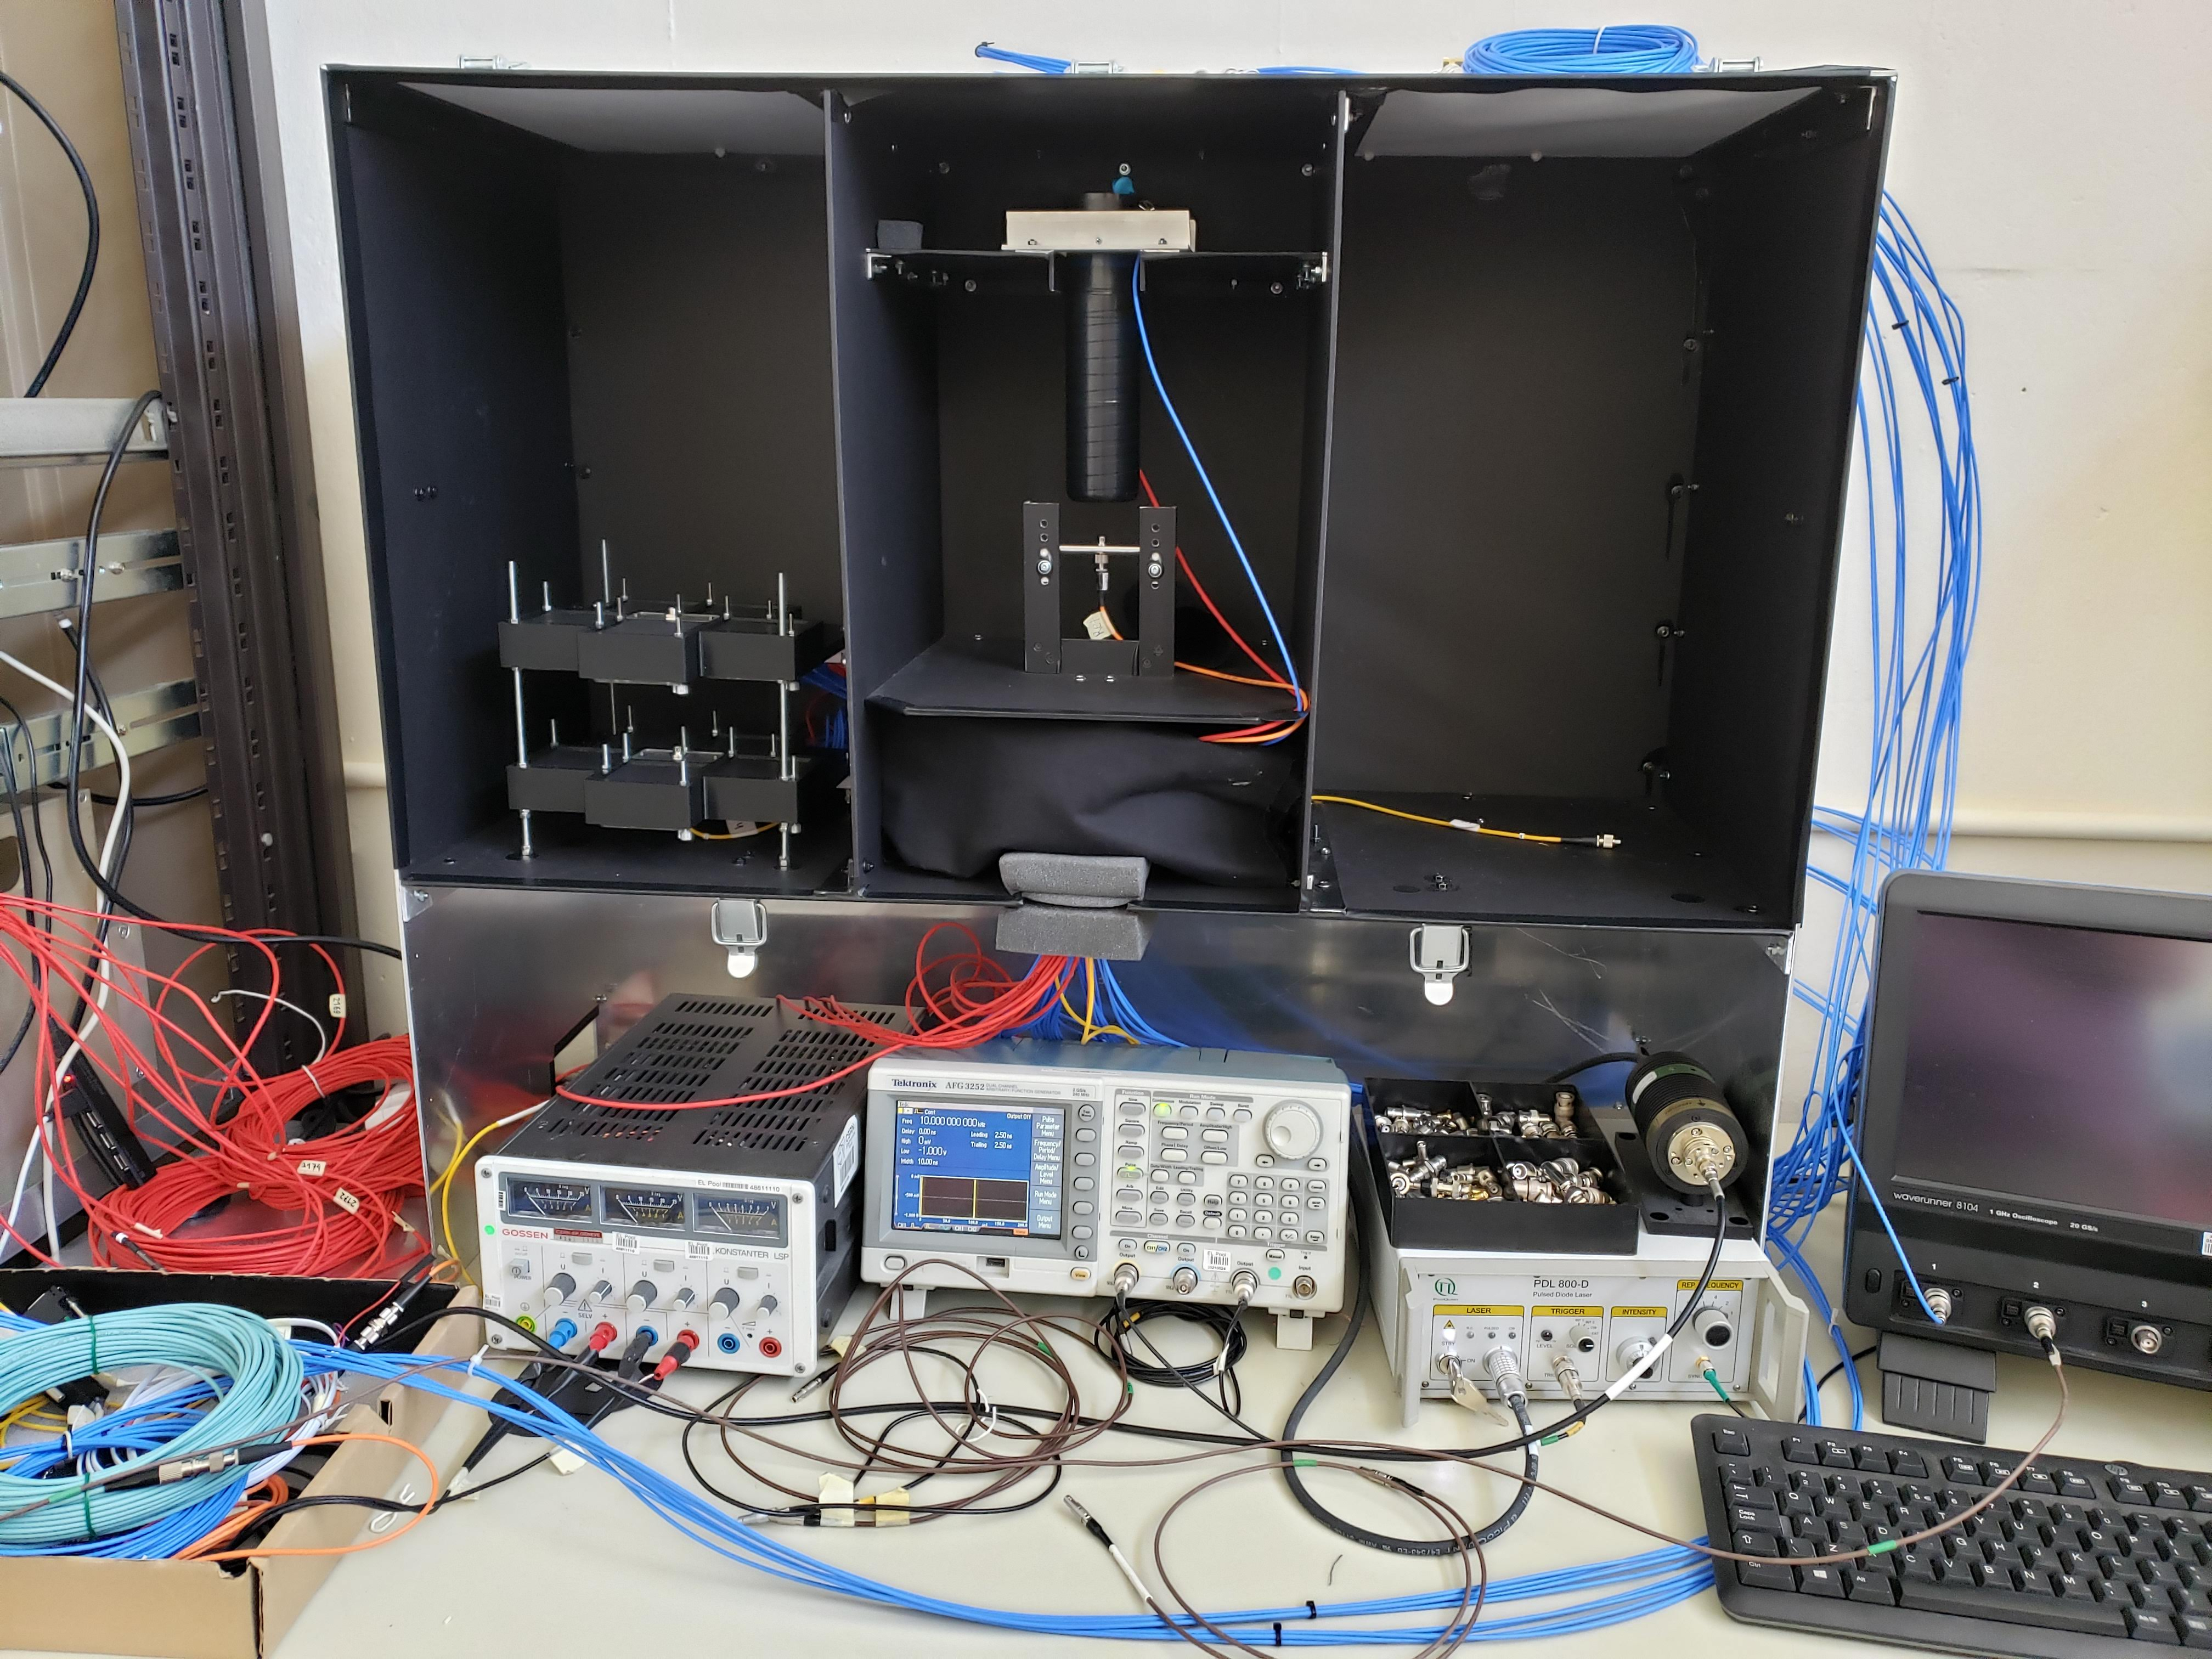
\includegraphics[width=0.8\textwidth]{figures/FIT/PMT_Test_apparatus.jpg}
    \caption{MCP-PMT Testing apparatus at the ALICE FIT Lab. Laser pulser, HV power supply, oscilloscope, function generator, isolating aluminum frame for light-tight data collection.}
    \label{fig:PMT_Testing_Apparatus}
\end{figure}

\begin{figure}[H]
  \centering
  \subfloat[T0+ C-side test assembly for MCP-PMTs in the FIT Lab.]{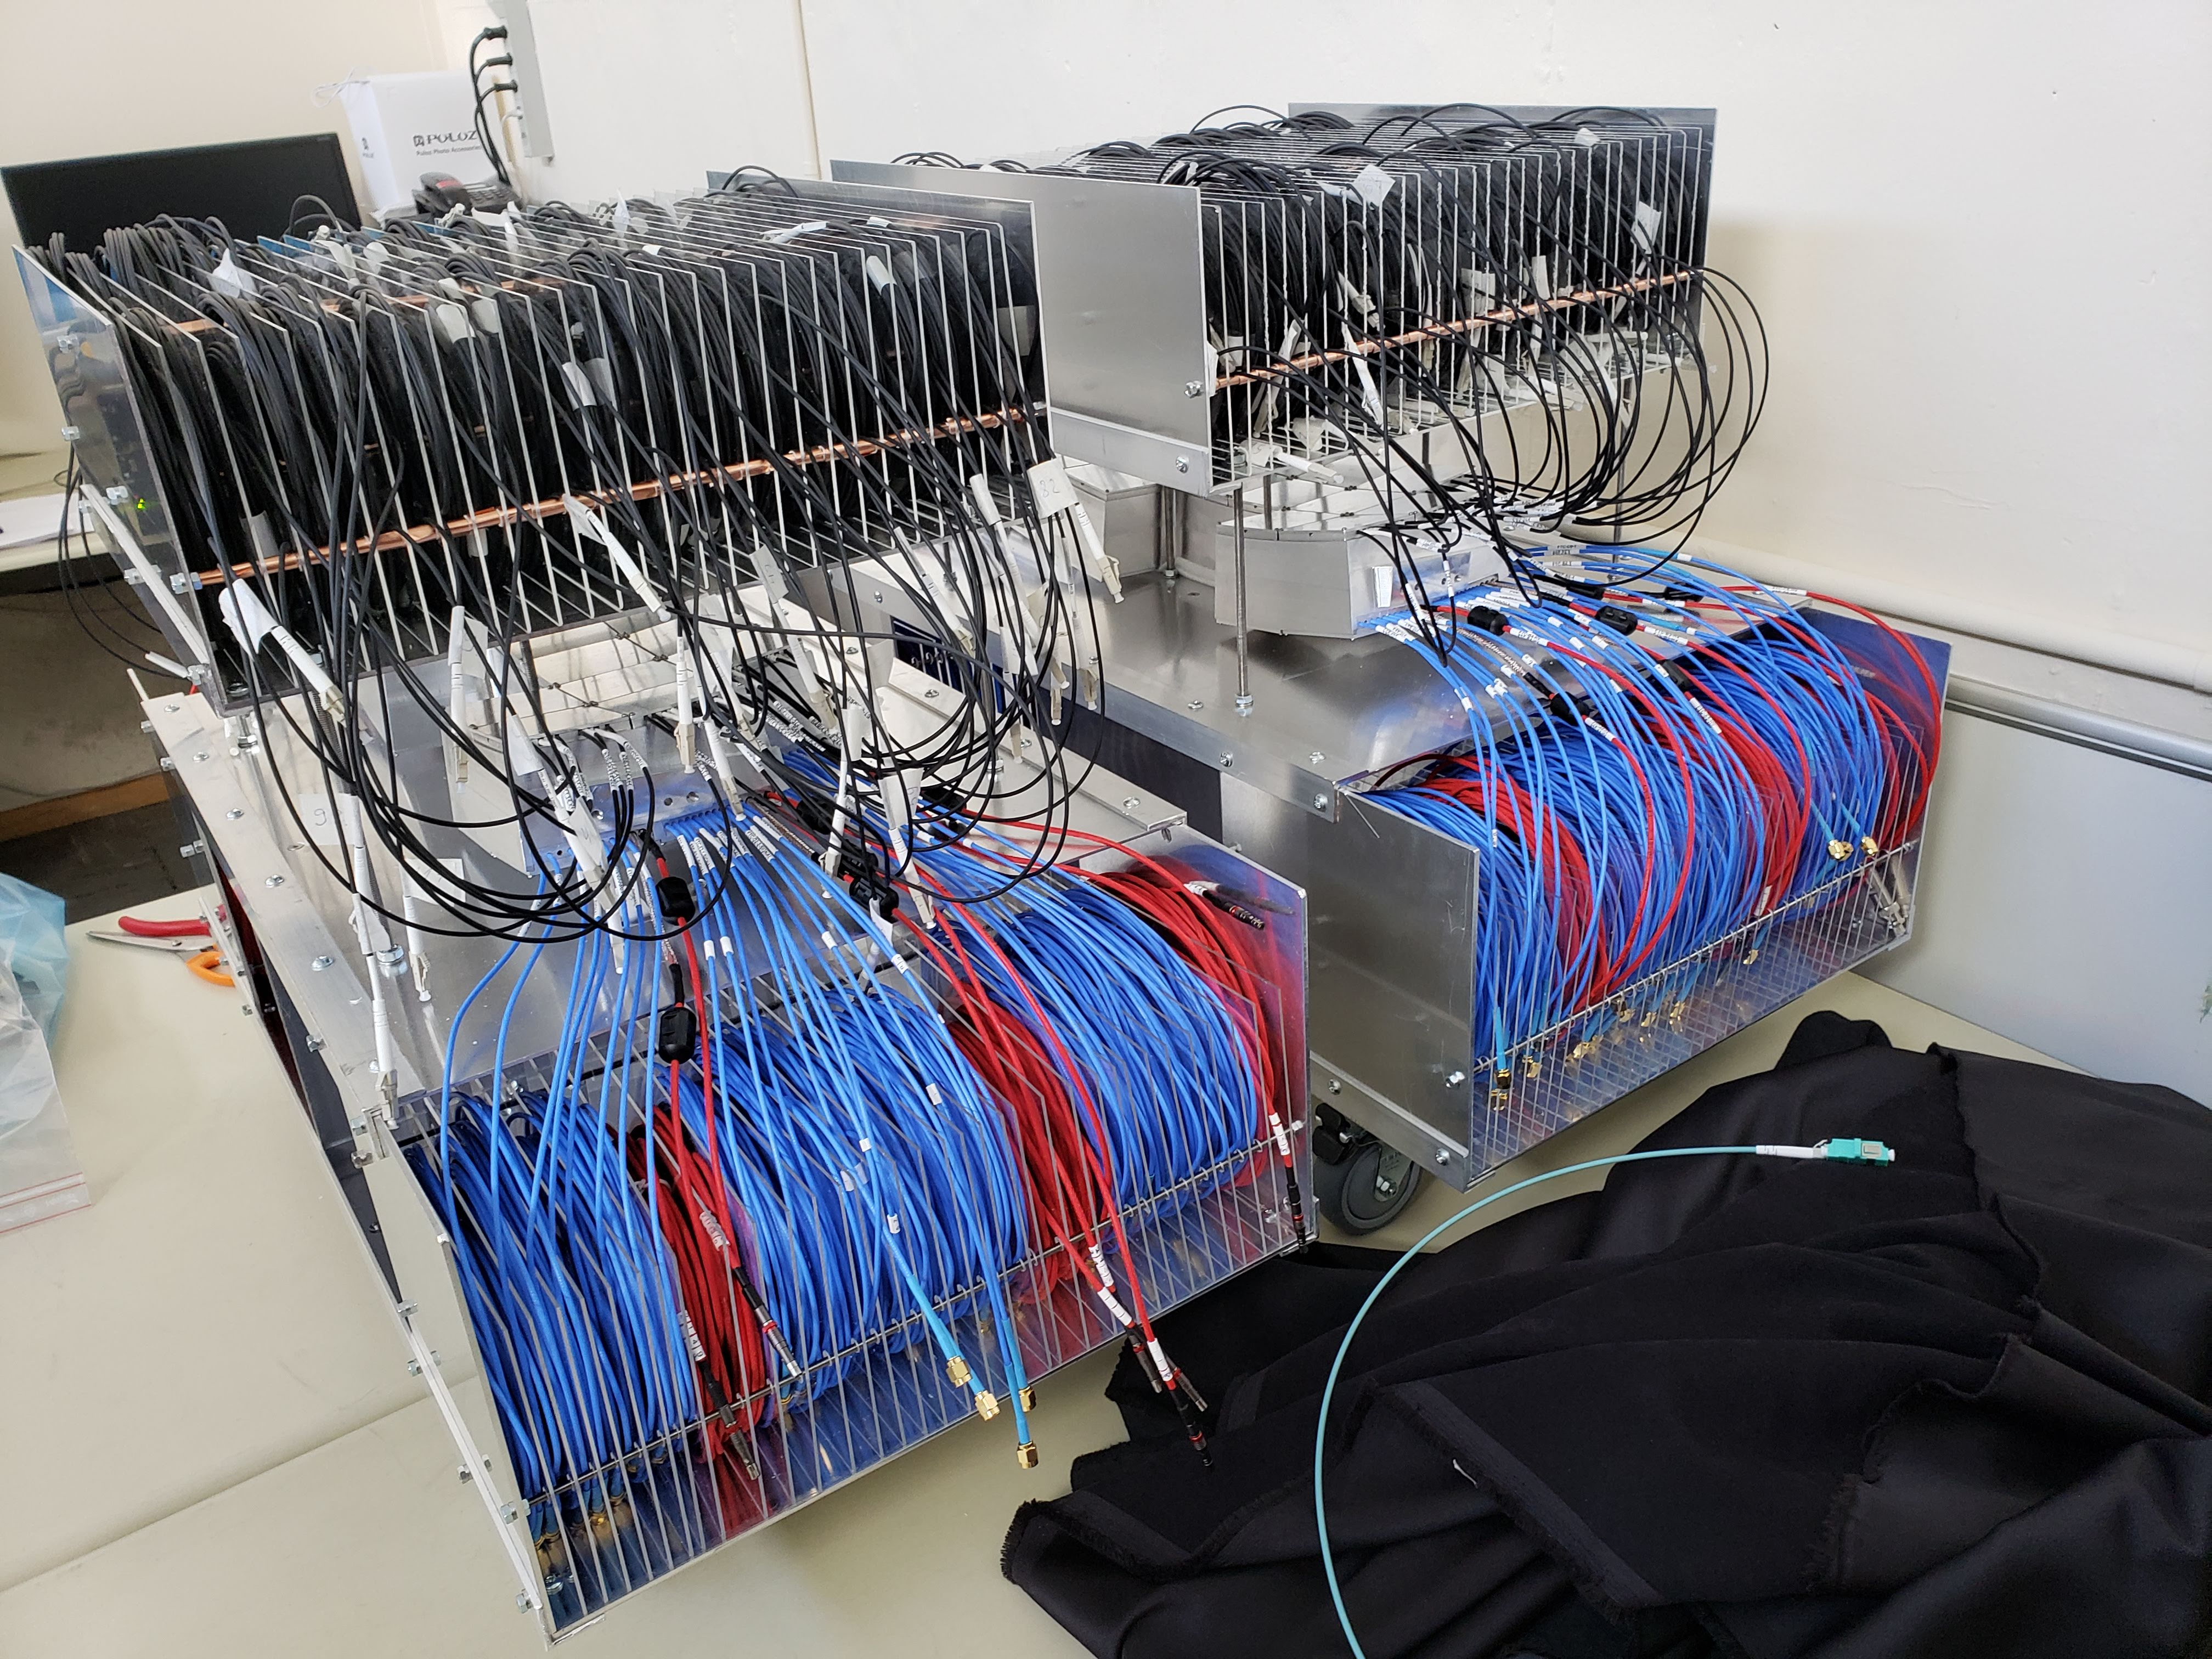
\includegraphics[width=0.4\textwidth]{figures/FIT/FT0_C_TestBench.jpg}\label{fig:FT0C_TestAssembly}}
  \hfill
  \subfloat[Side view of T0+C test assembly, showing the Aluminum support structure that holds the quartz radiators and PMTs.]{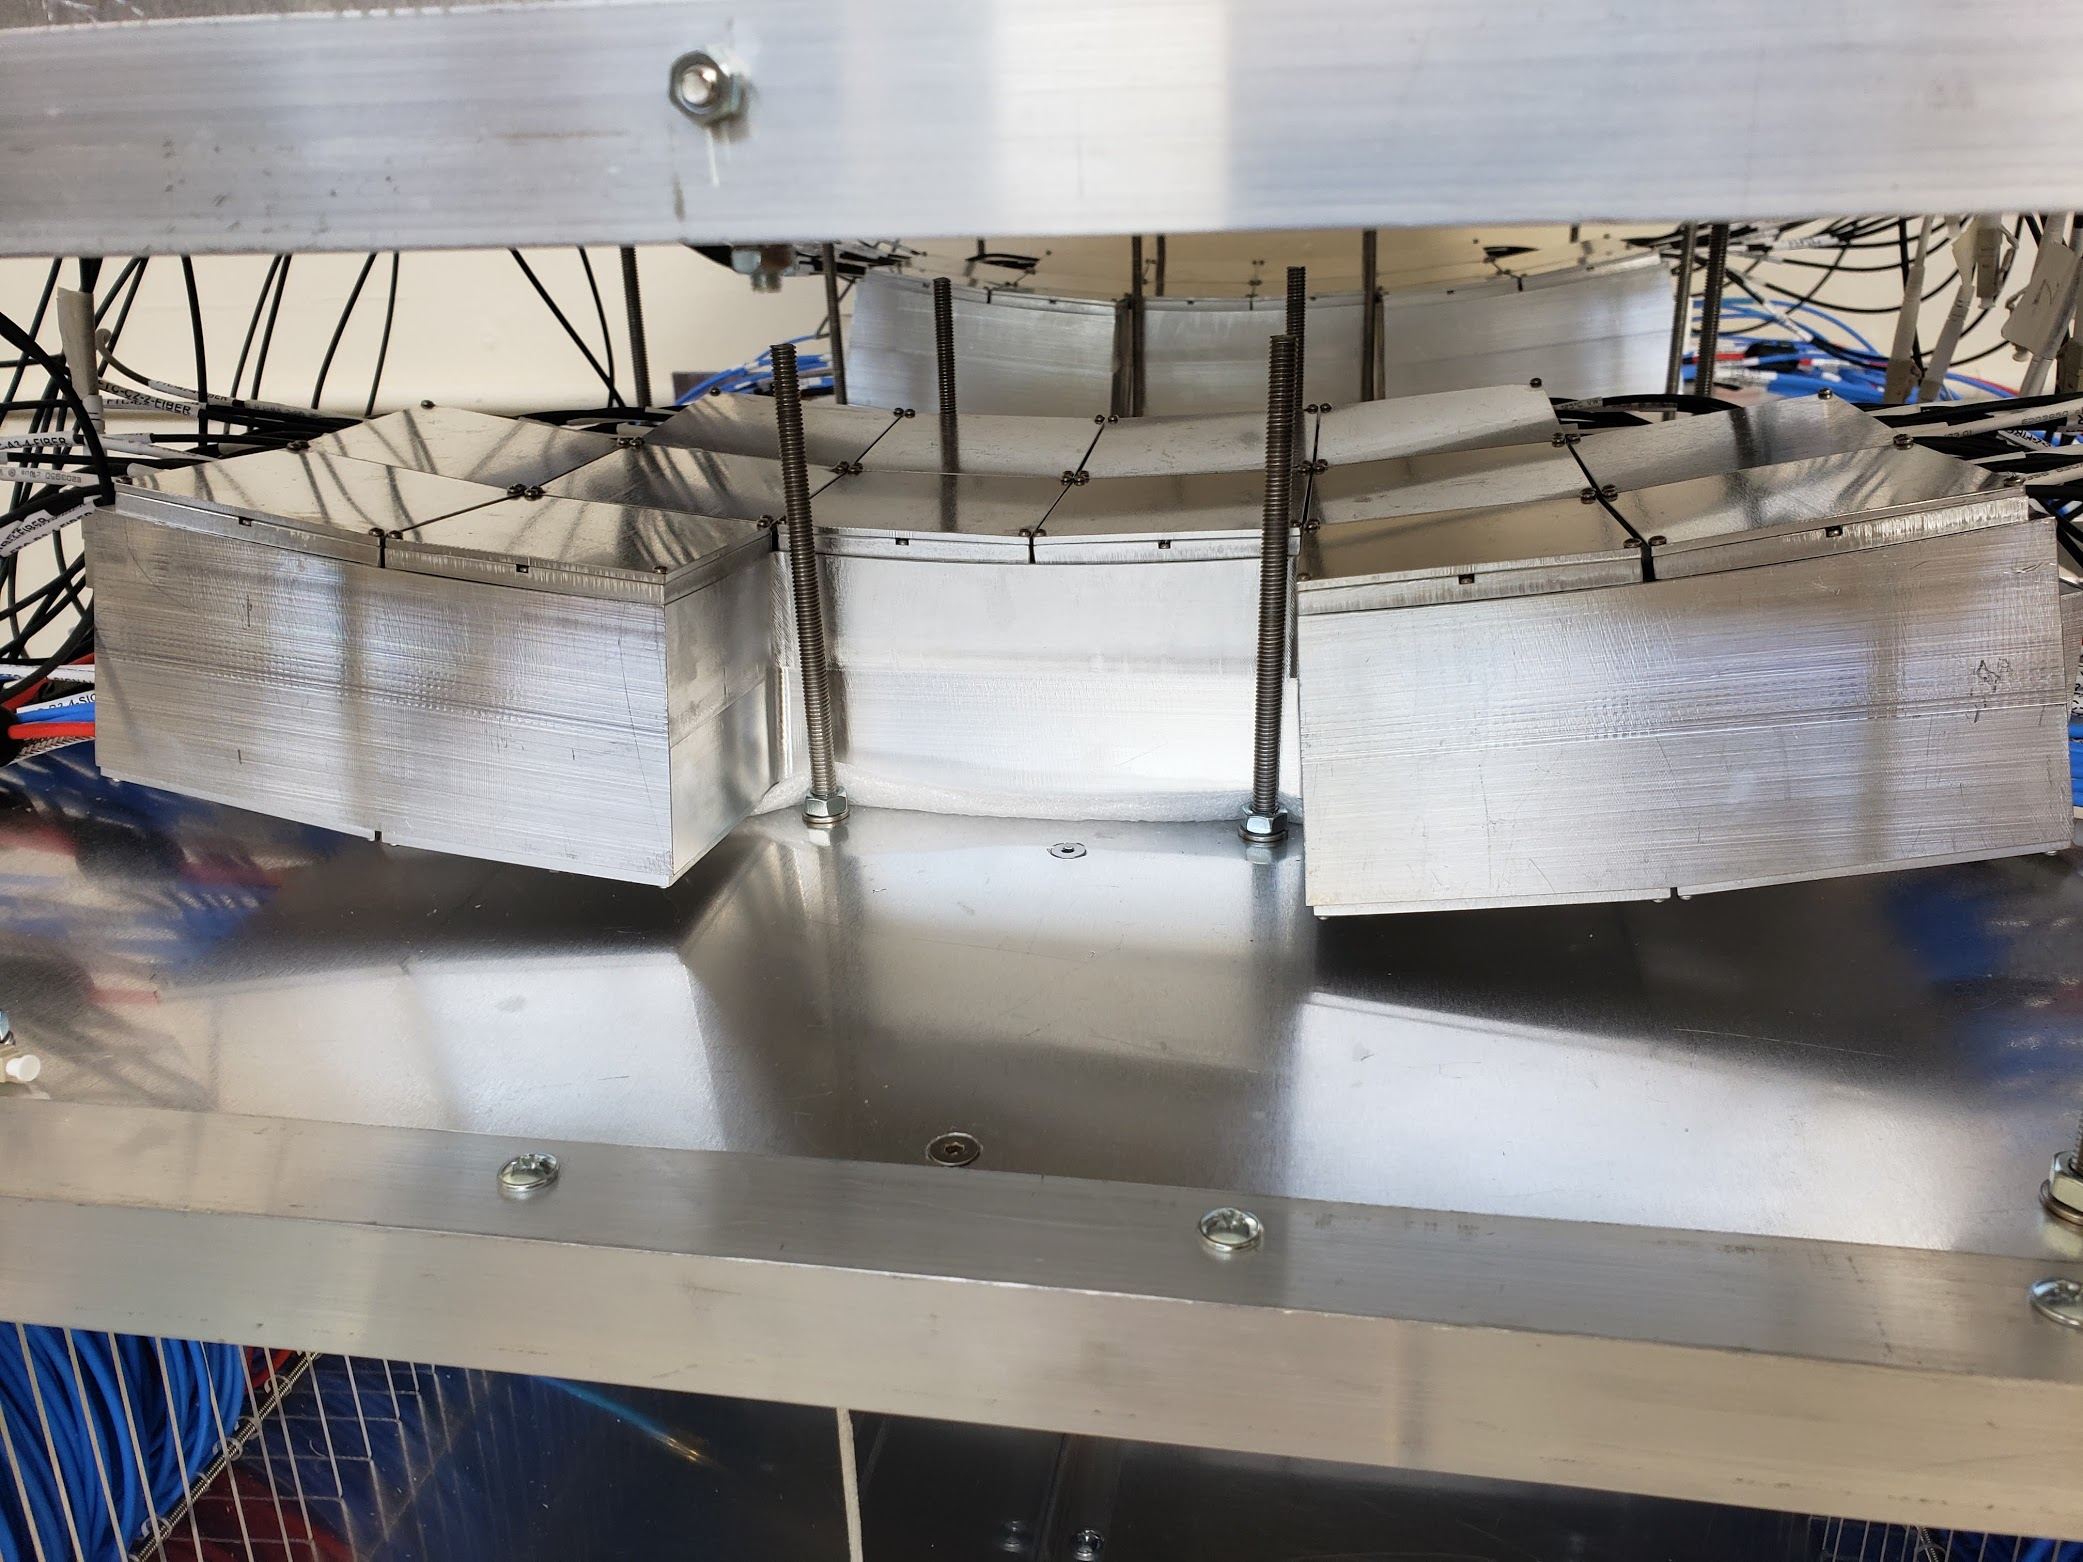
\includegraphics[width=0.4\textwidth]{figures/FIT/FT0_C_half.jpg}\label{fig:FT0C_In_Al_Structure}}
  \caption{FIT T0+ C-side in the FIT lab for MCP-PMT testing.}
\end{figure}


\begin{figure}[H]
    \centering
    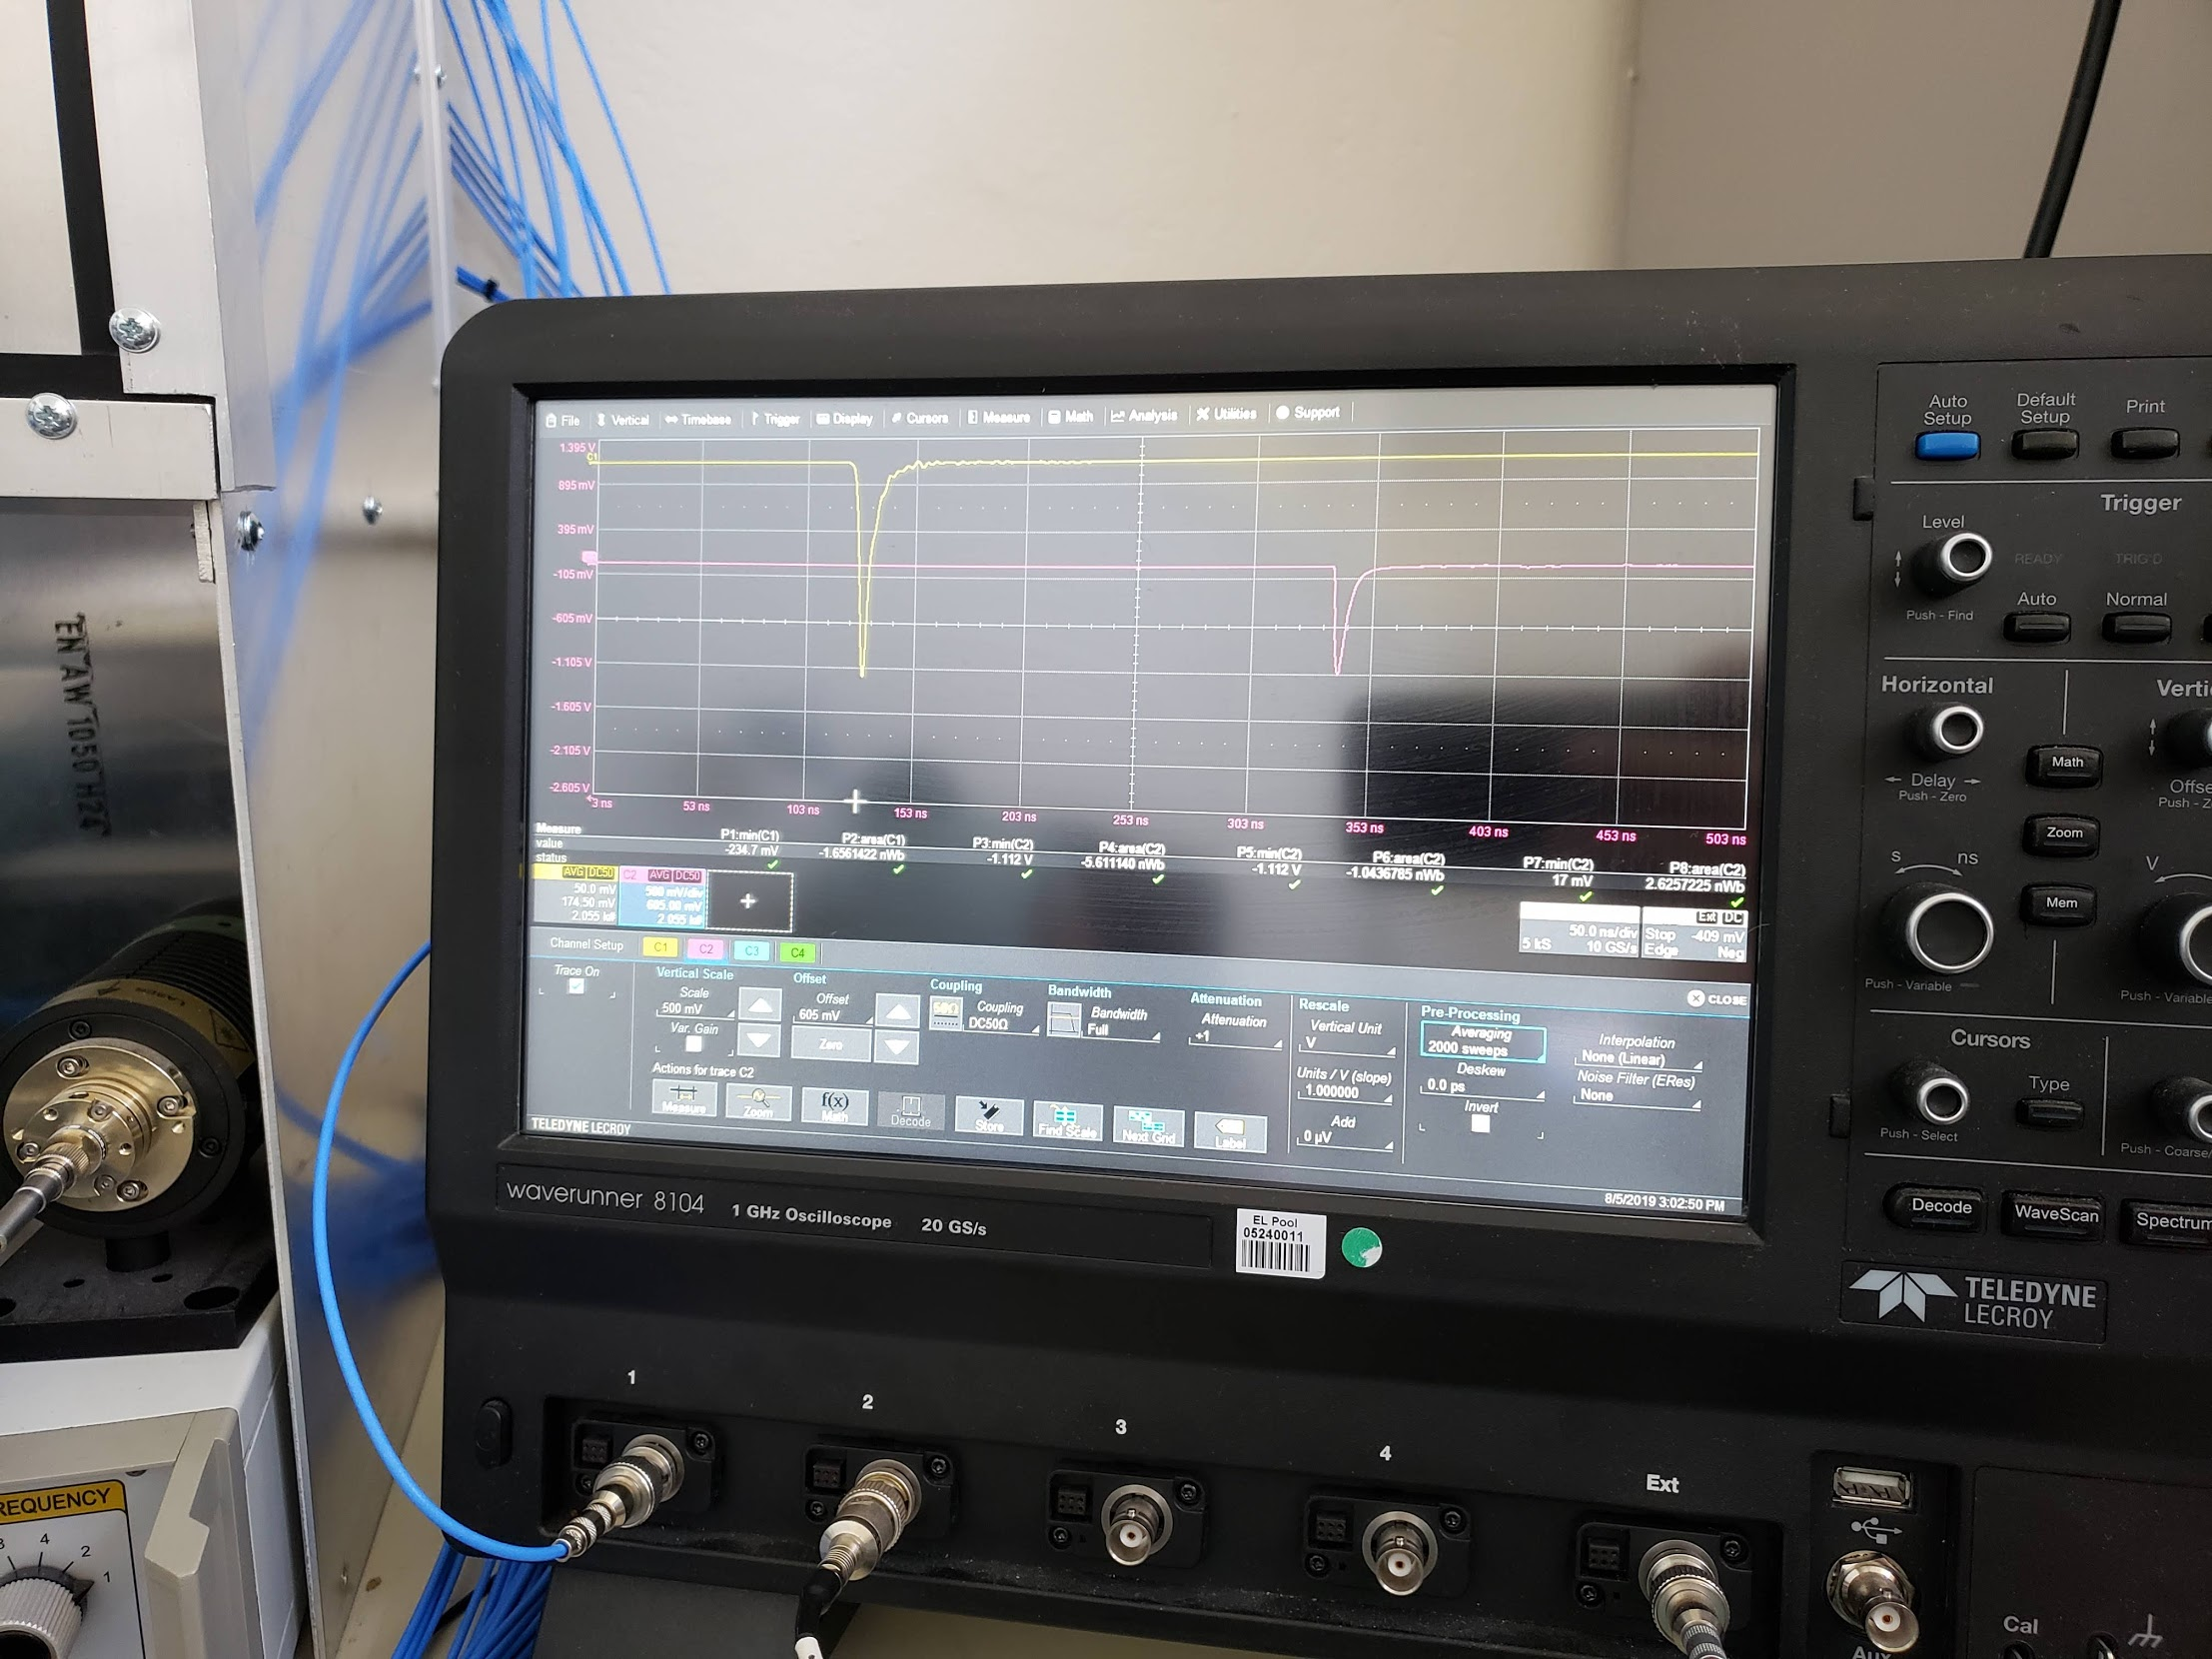
\includegraphics[width=0.8\textwidth]{figures/FIT/PMT_test_pulse.jpg}
    \caption{Oscilloscope trace of a current spike from a reference PMT (yellow) and the test PMT (pink).}
    \label{fig:my_label}
\end{figure}



\chapter{$O^2$ Simulations of FT0-A}
The ALICE Online-Offline Computing System $O^2$ has built-in simulation capabilities which include the generation of events and the transport of particles from the primary vertex. Using the FIT detector geometry in a simulation, we can determine the number of particles that can be detected using FIT sensitive components, and the number of secondary particles that contribute to the noise of other detectors. $O^2$ handles simulation data very similarly to true event data in the form of \textit{digits}, which only keep the location and energy deposition in the detector channel. Using this information, simulations can be used to inform live track reconstruction, background estimation, and particle identification. 


\sectionWithFixedHeader{Monte Carlo Event Simulations and Detector Geometry}{MC Simulations}

Simulations of particle physics interactions consist of three main components of simulation: event generation, particle transport, digitization. These elements of simulation are supported by specialized software that is optimized for each task. Monte Carlo simulations use computational approaches for randomized independent events; the inherent statistical nature of the events is evinced by the experimentally determined probability distribution functions, which are sampled randomly for each event. 

\subsection{Event Generation}
 Particles in the LHC are circulated in "bunches", which have a wide distribution of momentum and rapidity. To simulate the stochastic nature of events in ALICE, $O^2$ uses a Monte Carlo event generator such as PYTHIA for p-p collisions \cite{PYTHIA} or HIJING for Pb-Pb collisions \cite{HIJING}, and others for testing different kinds of physics.
 
\subsection{Particle Transport}
Particle transport is important for the next step in simulation. After an event is generated, particles are propagated away from the interaction point using experimentally determined probability distributions to simulate the passage of generated particles through the detector, modeling their energy loss in the material description of the detector.  To do this we need a geometric description of the detector. Particle transport must be optimized to handle the high volume of data produced by the particles as they pass through the detector description, which is achieved using the GEANT4 (for GEometry ANd Tracking) package\cite{Geant4}. GEANT4 has a multi-threading library that satisfies the $O^2$ speed requirements. Along with high particle transport efficiency, GEANT4 has compatibility with ROOT\cite{ROOT} geometry capabilities that allow for construction of the ALICE detector geometry in simulation.  Figure \ref{fig:GEANT_Geometry} shows the LHC Run 1 ALICE detector rendered in GEANT4 using the ROOT geometry package.  GEANT4 helps to accurately track which of the detectors are hit, which materials a particle travels through, and how much energy is deposited at each step of the transport process.  All of this information can be packaged into composite signals that mimic the information that would be provided in a real detector operating in beam.  For this project, the FT0-A support structure geometry has been implemented and will be described in the next section.

\subsection{Digitization and Reconstruction}

As particles are propagated through detector geometry, interactions that deposit energy into a material are considered \textit{hits}. Hits are implemented to contain all information from the interactions, acting as Maxwell's Demon \cite{MaxwellDemon} with a ledger of all vertices and branches that precede the hit. This information is convolved with the granularity, live-time, signal shape, and ADC characteristics of the electronics used in detector hardware, which comes from experimental hardware tests and is included in the simulation implementation. Using information from the hits and detector fidelity tests, \textit{digits} are computed. Digits contain the same information as real experimental signals and can be used to reconstruct tracks left in the detectors. This is done by comparing reconstructed tracks using the digits and experimental data, then matching reconstructed tracks with the simulated hits. 

\begin{figure}[H]
    \centering
    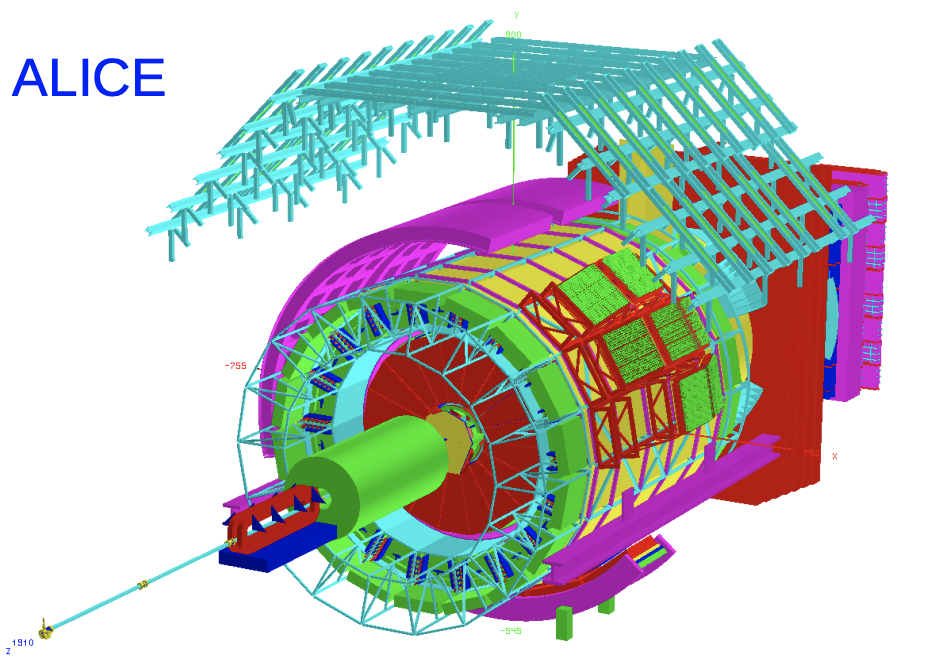
\includegraphics[width=0.6\textwidth]{figures/ALICE/GEANT_Geometry.png}
    \caption{RUN 1 ALICE detector geometry implemented in Geant4\cite{alice_geant} }
    \label{fig:GEANT_Geometry}
\end{figure}


\sectionWithFixedHeader{FT0-A Aluminum Support Structure $O^2$ Implementation}{FT0-A Aluminum  Support}
CAD drawings of the final design for the FIT FT0-A support structure, shown in Figure \ref{fig:FT0_CAD}, were completed in summer of 2019, and the support structure needed to be included in the simulation geometry. Using ROOT's geometry description software, the structure was implemented into the $O^2$ FT0 class, and is now included in simulations of FT0.  Figure \ref{fig:FT0_Labels} shows the description of the detector component labeling scheme for FT0-A and FT0-C.

\begin{figure}[H]
    \centering
    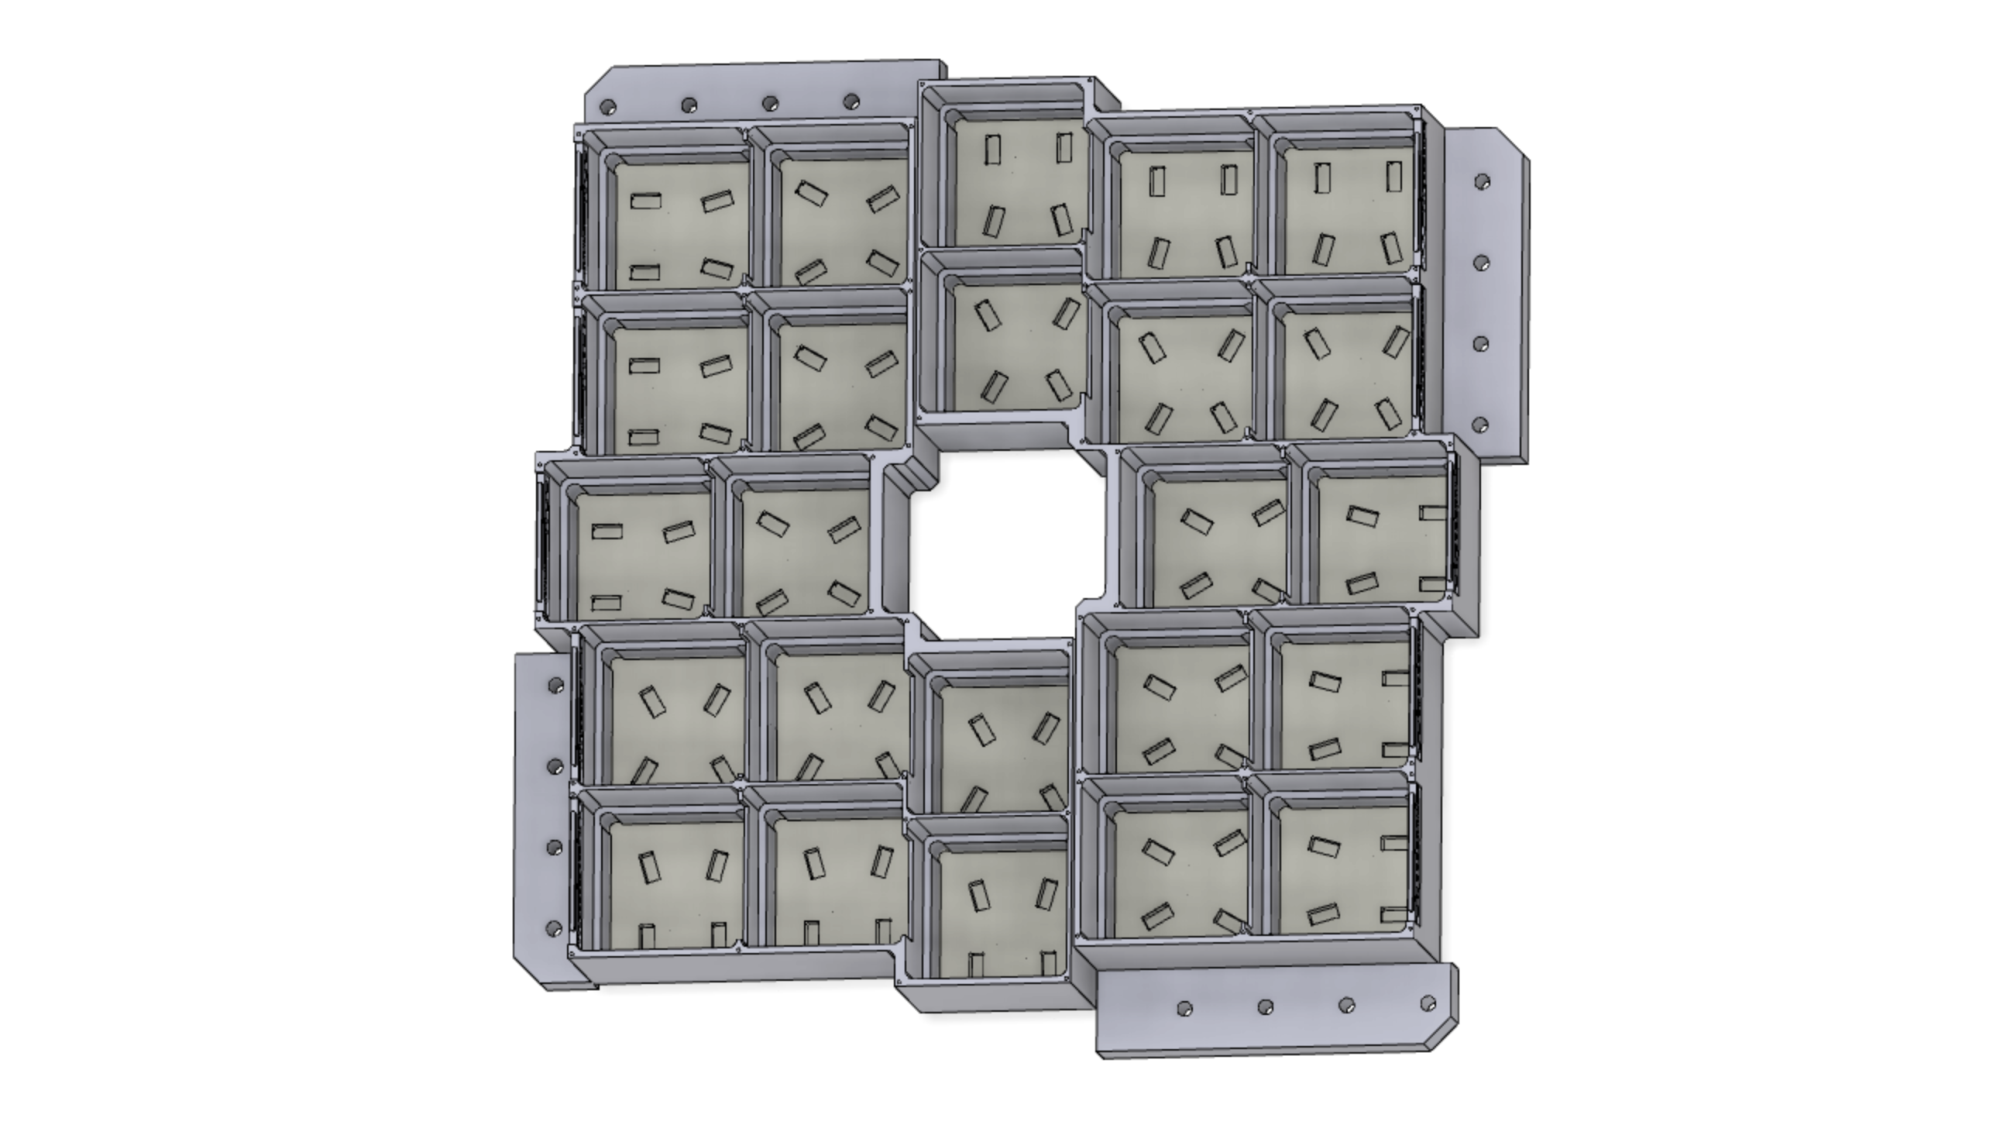
\includegraphics[width=0.6\textwidth]{figures/FIT/FIT_Support_Structure_CAD.pdf}
    \caption{CAD drawing of Aluminum support structure for FT0-A.}
    \label{fig:FT0_CAD}
\end{figure}

\begin{figure}[H]
    \centering
    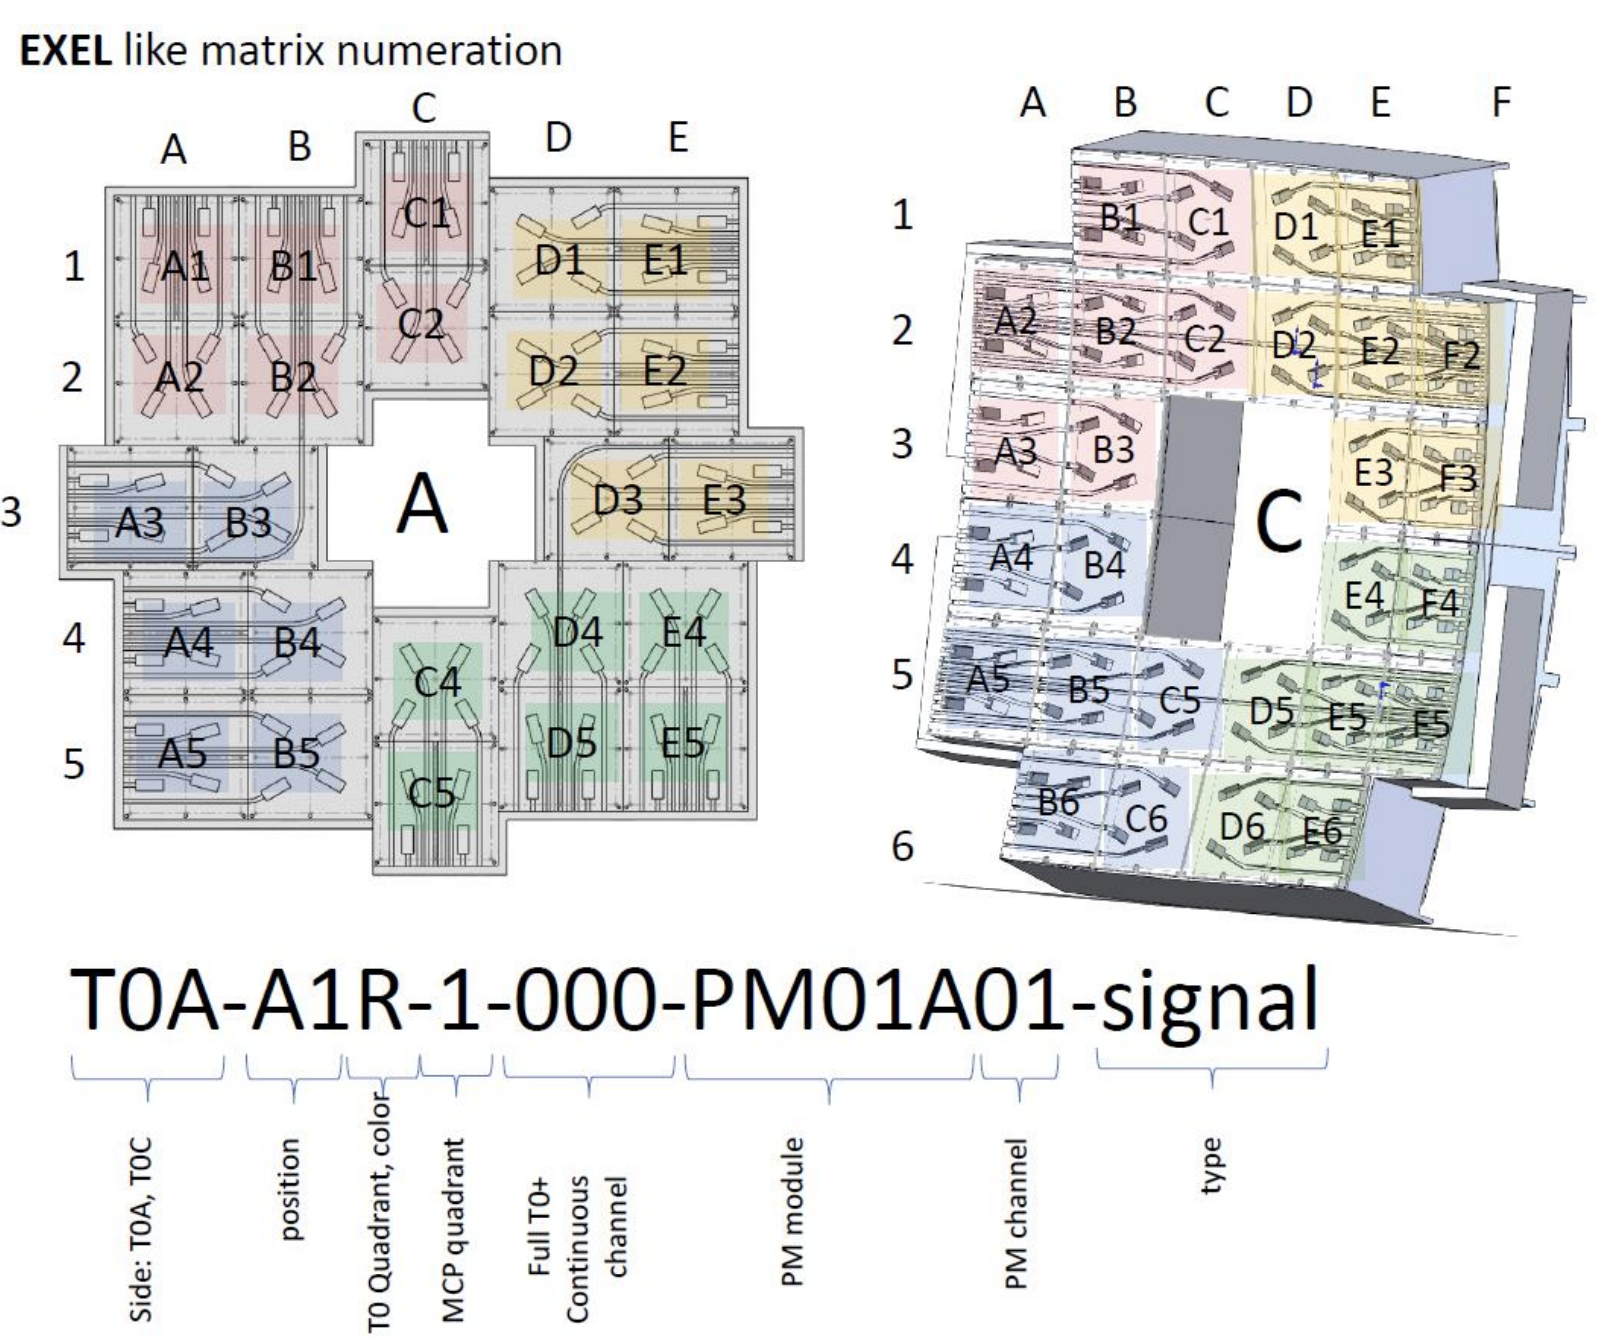
\includegraphics[width=0.6\textwidth]{figures/FIT/T0_Structure_and_Cell_Numbers.png}
    \caption{Aluminum support structure for FT0 A and C sides. Cells are enumerated by row and column.}
    \label{fig:FT0_Labels}
\end{figure}

\section{Results and Discussion}

After the FT0-A detector geometry was completed, a set of simulations of the sensitive components and the support structure for the FT0-A were run, using PYTHIA \cite{PYTHIA} in $O^2$.  Figure \ref{fig:FT0A-SensitiveComponents} shows the geometry of the sensitive components of the A-side detector, including the Cherenkov radiative crystals (Top) and MCP-PMTs (Bottom), coupled with optical grease.  Figure \ref{fig:HitHistogram} shows the location of all simulated hits in those sensitive components, as determined by the particle transport process in GEANT4. The next steps in this analysis include investigating the secondary particles produced in this simulation and evaluating their contribution to the noise in other detectors. This future work is described in Chapter 4.


\begin{figure}[H]
    \centering
    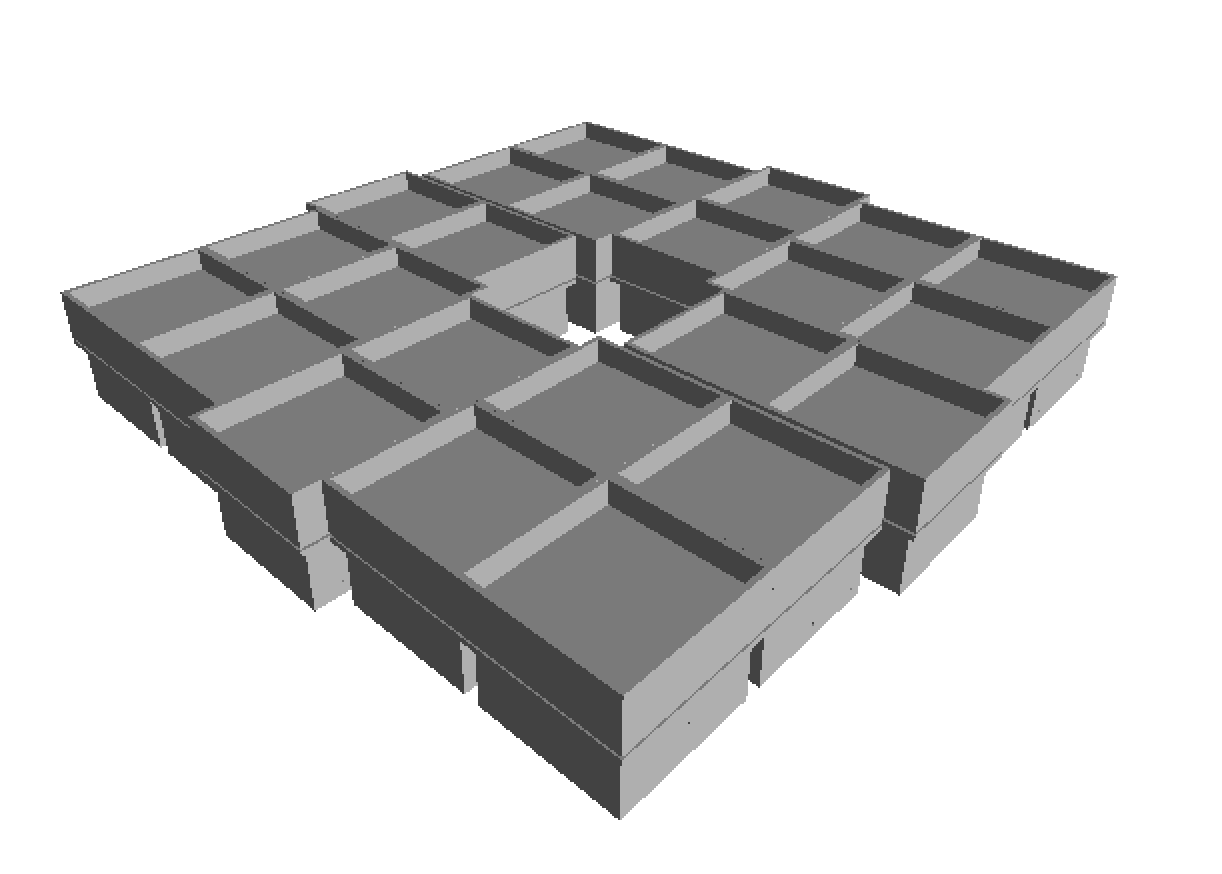
\includegraphics[width=0.8\textwidth]{figures/FIT/T0+_Sensitive_Components.png}
    \caption{Sensitive components for FT0-A. This includes the Cherenkov radiative crystals (Top) and MCP-PMTs (Bottom), coupled with optical grease}
    \label{fig:FT0A-SensitiveComponents}
\end{figure}

\begin{figure}[H]
    \centering
    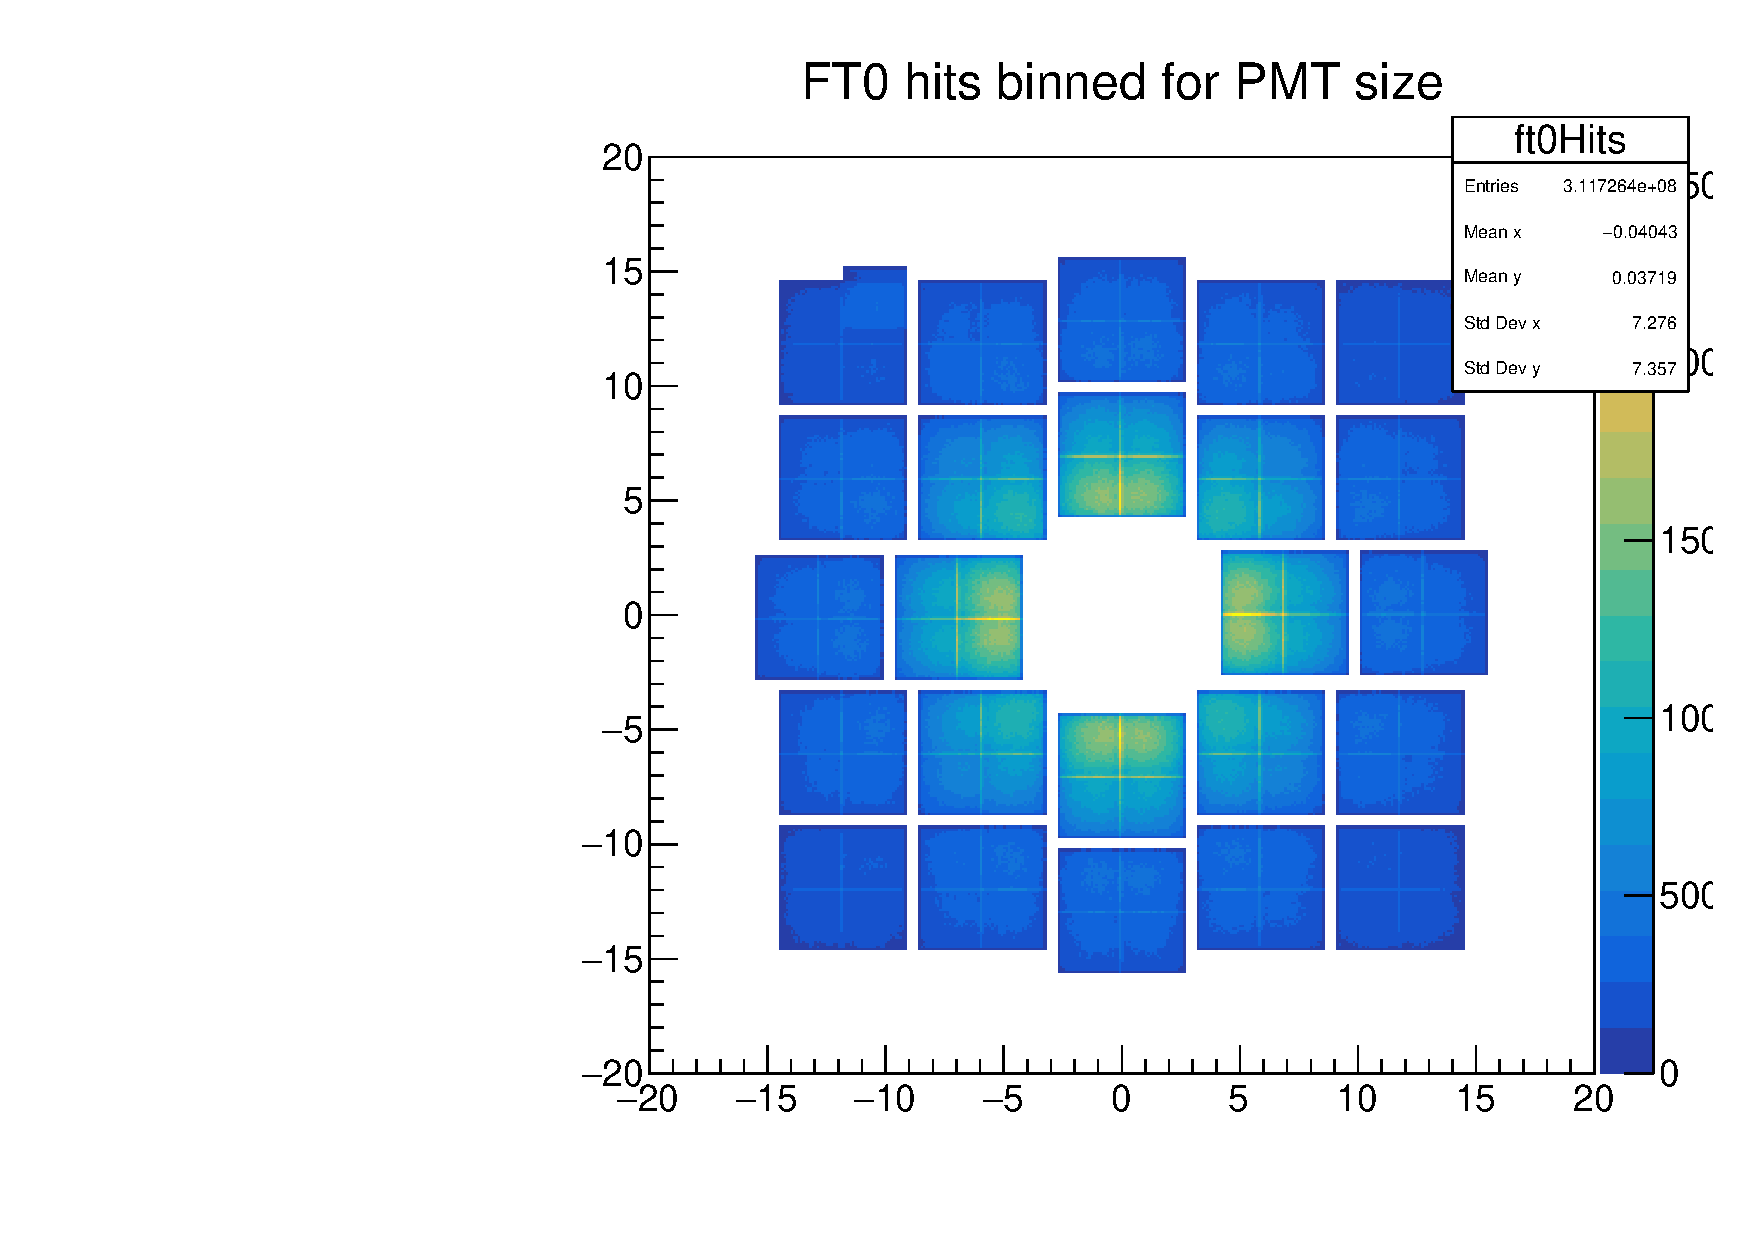
\includegraphics[width= 0.8\textwidth]{figures/analysis/T0+_Sensitive_Components.pdf}
    \caption{Histogram of energy deposited in the FT0-A sensitive components (``hits''), as simulated by GEANT4 particle transport. The MCPs nearest the beamline in p-p collisions end up most exposed due to low transverse momentum interactions.}
    \label{fig:HitHistogram}
\end{figure}

\chapter{Summary and Conclusion}

The CERN LHC Long Shutdown 2 is a scheduled maintenance and upgrade period for each of the experiments and the accelerator ring. During this period, the ALICE collaboration has been working on major upgrades, including the development of the Fast Interaction Trigger (FIT) detector. These upgrades include increased detector acceptance and resolution, as well as enhanced simulation capabilities using the $O^2$ Computing System. For this project, both hardware and software tasks in support of the FIT detector upgrade have been completed.  

Chapter 2 includes a summary of the FIT hardware, with an emphasis on the electronics of FIT T0+ (FT0). FT0 is a Cherenkov detector composed of quartz radiators and Micro-channel plate photomultipliers (MCP-PMTs) to detect particles from the interaction zone early enough to signal data acquisition in the rest of ALICE.  In the summer of 2019, high voltage electronics were assembled and tested in the ALICE FIT lab. Testing was done using a pulsed laser, which was split between a test MCP-PMT and a reference traditional PMT. By measuring the response of each MCP, the appropriate driving voltages and wiring order was determined. Logging these tests is useful because each MCP measures independently, so the crosstalk between channels is important to characterize.  These components have been assembled into a complete detector and will supply trigger signals to ALICE during LHC Run 3. 

Chapter 3 provides an overview of the software written to include an Aluminum support structure for FT0-A in simulations. This is useful for determining how the support structure will affect detector resolution and backgrounds. The software was implemented within the ALICE $O^2$ framework, an upgrade to the full ALICE data acquisition and reconstruction software that was necessary to handle the increased luminosity and data volumes expected in LHC Run 3. The geometry of the support structure was translated from CAD drawings into a geometrical description within ROOT. An example analysis is given in Chapter 3, including a histogram of the hits generated in the FT0-A sensitive components.


\section{Outlook and Future Work}

This thesis lays the groundwork for future Cal Poly Senior Projects, with opportunities extending in both hardware and software. Having assembled and tested the MCP-PMTs used in ALICE, the description of FIT hardware in Chapter 2 can be used to develop an introductory physics experiment: students can develop a testing apparatus similar to the one shown in Fig. \ref{fig:PMT_Testing_Apparatus} to become acquainted with electronics used in High Energy Physics. The software development in this thesis incorporated the Aluminum support structure into $O^2$ simulations and includes a basic example of ROOT analysis capabilities. Using the $O^2$ computing framework, students can run analysis tasks to determine the detector performance, acceptance, and background contributions. Specific examples of projects that will contribute to make all of ALICE Run 3 physics possible include 

\begin{itemize}
    \item digitizing the hits and analyzing the output to determine trigger efficiency, timing resolution for FT0-A
    \item investigating secondary particles generated in the FT0-A detector geometry that contribute background noise to other detectors
    \item completing the FT0-C support structure description and carrying out the same characterization tasks as for FT0-A
    \item implementing the geometric description of the additional material for cabling and electronics, then repeating the characterization tasks
\end{itemize}

Projects such as these are ideal for senior theses, as they are accessible and allow students to experience both the hardware and software elements of detector development in one of the most complex and cutting-edge experiments at the world's largest accelerator.
 
 
\newpage
\Urlmuskip=0mu plus 1mu\relax
\bibliographystyle{unsrt}
\bibliography{references}

\end{document}
